\documentclass[11pt]{article}

\usepackage[margin=1in]{geometry}
\usepackage[T1]{fontenc}
\usepackage{lmodern}
\usepackage{microtype}
\usepackage{amsmath,amssymb,amsfonts,amsthm,mathtools}
\usepackage{graphicx}
\usepackage{booktabs}
\usepackage{enumitem}
\setlist[enumerate]{leftmargin=.35in, itemsep=2pt, topsep=4pt}
\setlist[itemize]{leftmargin=.35in, itemsep=2pt, topsep=4pt}
\usepackage[numbers,sort&compress]{natbib}
\usepackage{xcolor}
\usepackage{pgfplots}
\pgfplotsset{compat=1.18}
\usetikzlibrary{pgfplots.groupplots}
\usepackage[colorlinks=true,linkcolor=blue!55!black,citecolor=teal!60!black,urlcolor=blue!55!black]{hyperref}
\usepackage[nameinlink,capitalize,noabbrev]{cleveref}

\hypersetup{
  pdftitle={Sharp Growth and Outlier-Robust Local Recovery in l1 Max-Linear Regression},
  pdfauthor={Haixin Huang},
  pdfsubject={Research Preprint (Not Peer-Reviewed)},
  pdfkeywords={max-linear regression, robust statistical estimation, sharp growth, nonsmooth nonconvex optimization, least absolute deviations, adversarial outliers, formal verification}
}

% Theorem environments sharing a per-section counter (matches exact numbering across versions)
\theoremstyle{plain}
\newtheorem{theorem}{Theorem}[section]
\newtheorem{lemma}[theorem]{Lemma}
\newtheorem{proposition}[theorem]{Proposition}
\newtheorem{corollary}[theorem]{Corollary}
\theoremstyle{remark}
\newtheorem{remark}[theorem]{Remark}
\newtheorem{example}[theorem]{Example}

% TeX Live 2025/2026 cleveref + amsthm shared-counter alias fix
\AddToHook{env/lemma/begin}{\crefalias{theorem}{lemma}}
\AddToHook{env/proposition/begin}{\crefalias{theorem}{proposition}}
\AddToHook{env/corollary/begin}{\crefalias{theorem}{corollary}}
\AddToHook{env/remark/begin}{\crefalias{theorem}{remark}}
\AddToHook{env/example/begin}{\crefalias{theorem}{example}}

\newcommand{\creflastconjunction}{, and~}
\crefname{theorem}{Theorem}{Theorems}
\Crefname{theorem}{Theorem}{Theorems}
\crefname{lemma}{Lemma}{Lemmas}
\Crefname{lemma}{Lemma}{Lemmas}
\crefname{proposition}{Proposition}{Propositions}
\Crefname{proposition}{Proposition}{Propositions}
\crefname{corollary}{Corollary}{Corollaries}
\Crefname{corollary}{Corollary}{Corollaries}
\crefname{remark}{Remark}{Remarks}
\Crefname{remark}{Remark}{Remarks}
\crefname{section}{Section}{Sections}
\Crefname{section}{Section}{Sections}
\crefname{subsection}{Subsection}{Subsections}
\Crefname{subsection}{Subsection}{Subsections}

\numberwithin{equation}{section}

% Mathematical macros
\newcommand{\R}{\mathbb{R}}
\newcommand{\N}{\mathbb{N}}
\newcommand{\E}{\mathbb{E}}
\newcommand{\Prob}{\mathbb{P}}
\newcommand{\Sph}{\mathbb{S}}
\newcommand{\ind}{\mathbf{1}}
\newcommand{\ip}[2]{\langle #1, #2 \rangle}
\newcommand{\norm}[1]{\|#1\|}
\newcommand{\abs}[1]{|#1|}
\newcommand{\dist}{\operatorname{dist}}
\newcommand{\argmin}{\operatorname*{arg\,min}}
\newcommand{\argmax}{\operatorname*{arg\,max}}
\newcommand{\sign}{\operatorname{sign}}
\newcommand{\Fnorm}[1]{\|#1\|_F}
\newcommand{\Lonenorm}[1]{\|#1\|_{1,2}}
\newcommand{\opnorm}[1]{\|#1\|_{\mathrm{op}}}

\title{\bfseries Sharp Growth and Outlier-Robust Local Recovery in $\ell_1$ Max-Linear Regression\thanks{Research preprint (not peer-reviewed). Companion Supplementary Materials (\texttt{supplement.pdf}), Lean~4 formal verification package, and reproducible experiment scripts are archived alongside this manuscript.}}

\author{Haixin Huang\thanks{Independent Researcher, Naples, Italy. Email: \texttt{huanghaixin061028@gmail.com}. ORCID: \url{https://orcid.org/0009-0005-5243-0680}.}}

\date{November 22, 2026}

\begin{document}

\maketitle

\begin{abstract}
We analyze the statistical and variational geometry of the nonconvex, nonsmooth $\ell_1$ empirical risk for max-linear regression, $f(\beta) = \frac{1}{m}\sum_{i=1}^m |y_i - \max_{1 \le j \le r} \ip{a_i}{\beta_j}|$, under i.i.d.\ standard Gaussian covariates $a_i \sim \mathcal{N}(0, I_d)$ and sparse adversarial corruptions. Unlike squared-$\ell_2$ max-affine estimators, which break down under gross outliers and suffer from a $\Theta(\pi_{\min}^3)$ active-cone Gram eigenvalue bottleneck, the $\ell_1$ risk is non-weakly-convex yet exhibits favorable first-order geometry. Our main result proves that for any $r \ge 2$ and any fixed oblivious outlier support of fraction $\alpha \in [0, 1/2)$, with high probability $f$ satisfies uniform macroscopic sharp growth $f(\beta) - f(\beta^*) \ge \frac{(1-2\alpha)\alpha_{\min}}{4}\Lonenorm{\beta - \beta^*}$ and global $2$-Lipschitzness simultaneously for all (possibly unbounded, data-dependent) corruption magnitudes, with explicit constants independent of the separation condition number $\kappa = \Delta_{\max}/\Delta_{\min}$ and free of $\log(m/d)$ factors. This resolves the quantitative Gaussian sharp-growth question left open by Charisopoulos and Davis (2024) in the local macroscopic regime, while a matching finite-sample converse shows $\alpha < 1/2$ is sharp under oblivious support. We further prove a closed-form $r = 2$ population remainder bound yielding the global, scale-free lower bound $F(\beta) \ge \frac{\sqrt{2}-1}{\sqrt{\pi}}\dist(\beta, X_{\mathrm{pop}}^*)$ and a dimension-free Gaussian bathtub inequality establishing a $\Theta(\pi_j^2)$-versus-$\Theta(\pi_j^3)$ conditioning advantage of $\ell_1$ over $\ell_2$ regression. Core statistical and geometric theorems are additionally machine-checked in Lean~4.

\medskip
\noindent\textbf{Keywords:} max-linear regression, robust statistical estimation, sharp growth, nonsmooth nonconvex optimization, least absolute deviations, adversarial outliers, formal verification.

\smallskip
\noindent\textbf{MSC 2020:} 62J02, 90C26, 49J52, 62F35, 68V15.
\end{abstract}

% ============================================================================
\section{Introduction}
\label{sec:intro}
% ============================================================================

Estimating a convex piecewise-linear function from high-dimensional observations is a canonical structured nonconvex problem in mathematical data science. In \emph{max-linear regression}, the response is modeled as the pointwise maximum of $r$ linear predictors:
\begin{equation}
  \label{eq:model}
  \hat y(a; \beta) := \max_{1 \le j \le r} \ip{a}{\beta_j},
  \qquad a \in \R^d,\quad \beta = (\beta_1, \dots, \beta_r) \in \R^{r \times d}.
\end{equation}
Applications include convex piecewise-linear approximation \cite{magnani2009convex}, adaptive convex regression \cite{hannah2013multivariate}, and high-dimensional statistical parameter recovery \cite{ghosh2022maxaffine,kim2024convex,kim2024firstorder,kanj2026sparse,kanj2026doma}. Given $m$ covariate-response pairs $(a_i, y_i)_{i=1}^m$, we study the least absolute deviations ($\ell_1$) empirical risk
\begin{equation}
  \label{eq:emp-loss}
  f(\beta) := \frac{1}{m}\sum_{i=1}^m \bigl|y_i - \hat y(a_i; \beta)\bigr|,
\end{equation}
with optimal value $f^* := \inf_{\beta \in \R^{r\times d}} f(\beta)$ and solution set $X^* := \argmin_{\beta \in \R^{r \times d}} f(\beta)$.

\paragraph{Robust statistical recovery and nonsmooth sharpness.}
Existing high-dimensional recovery theory for general $r$-component max-linear, max-affine, and difference-of-max-affine regression focuses predominantly on the squared $\ell_2$ loss under sub-Gaussian noise---covering alternating minimization \cite{ghosh2022maxaffine}, convex programming \cite{kim2024convex}, first-order gradient methods \cite{kim2024firstorder}, sparse estimation \cite{kanj2026sparse}, and adaptive block gradient descent \cite{kanj2026doma}. While these analyses achieve $O(d \cdot \operatorname{poly}(r, \pi_{\min}^{-1}))$ sample complexity, squared-$\ell_2$ estimators break down under a single gross outlier, often depend on the pairwise separation condition number $\kappa := \Delta_{\max}/\Delta_{\min}$, and are constrained by a $\Theta(\pi_{\min}^3)$ active-cone Gram eigenvalue bottleneck.

To achieve resilience against gross sparse corruptions, it is natural to turn to the $\ell_1$ objective~\eqref{eq:emp-loss}. In nonsmooth nonconvex estimation, local recovery and fast first-order convergence are governed by \emph{local sharp growth} (metric subregularity): on a neighborhood $U$ of a ground-truth parameter $\beta^* \in X^*$,
\begin{equation}
  \label{eq:sharp-growth}
  f(\beta) - f^* \ge \mu\,\dist(\beta, X^*) \qquad \forall \beta \in U,
\end{equation}
with modulus $\mu > 0$. Combined with global $L$-Lipschitzness,~\eqref{eq:sharp-growth} enables linear convergence of Polyak-type \cite{polyak1969minimization} and geometrically decaying subgradient schemes \cite{davis2018subgradient,davis2024stochastic} at a dimension-free rate determined by $L/\mu$. For \emph{weakly convex} objectives such as quadratic $\ell_1$ phase retrieval \cite{duchi2019solving,davis2020nonsmooth} and $\ell_1$ low-rank matrix recovery \cite{charisopoulos2021lowrank}, this sharp-growth paradigm yields strong outlier-robust statistical guarantees.

By contrast,~\eqref{eq:emp-loss} is \emph{not weakly convex} in general (\cref{prop:non-weak-convex}): an under-predicted sample ($\hat y(a_i; \beta) < y_i$) at an active tie produces a concave V-shaped kink of curvature $-\infty$. To address non-weakly-convex sharp problems, Charisopoulos and Davis \cite{charisopoulos2024superpolyak} established local linear convergence of \texttt{PolyakSGM} and local superlinear convergence of \texttt{SuperPolyak} under sharp growth~\texttt{(A1)} and $(b)$-regularity~\texttt{(A2)} ($|f(x) + \ip{v}{y - x} - f^*| \le C_{(b)}\norm{y - x}^{1 + \eta}$ for $v \in \partial f(x), y \in P_{X^*}(x)$). In Section~5.2.2 of \cite{charisopoulos2024superpolyak}, they observed rapid dimension-independent convergence on Gaussian $\ell_1$ max-linear regression, noted that semialgebraicity implies~\texttt{(A2)} whenever the solution set is isolated, and explicitly left the verification of~\texttt{(A1)} open.

\paragraph{Clarifying deterministic versus statistical sharpness.}
For any \emph{fixed} finite dataset $(a_i, y_i)_{i=1}^m$, qualitative local sharpness~\eqref{eq:sharp-growth} holds unconditionally for some data-dependent $\mu > 0$ and neighborhood $U$ by classical polyhedral error bound theory \cite{hoffman1952approximate,robinson1981some,gowda1996analysis,pang1997error,dolgopolik2023nonlocal} (\cref{prop:deterministic-eb}). However, Hoffman-type constants degrade arbitrarily with the data, and under Gaussian designs in dimension $d \ge 2$ the naive active-set stability radius around $\beta^*$ (for $r = 2$) collapses uniformly as $\Theta_{\Prob}(\norm{v}_2/(m\sqrt{d})) \to 0$ whenever $m\sqrt{d} \to \infty$ (\cref{prop:stab-decay}). The substantive statistical question is therefore establishing high-probability sharp growth~\eqref{eq:sharp-growth} with a \emph{dimension-free} modulus $\mu$ on a \emph{macroscopic} radius $\rho$ independent of $(m, d)$, together with local isolation of $\beta^*$ in $X^*$.

\paragraph{Related $\ell_1$ regression and phase-retrieval literature.}
Deterministic piecewise-linear $\ell_1$ optimization has been studied for Powell's censored LAD estimator \cite{powell1984censored,womersley1986censored} (one free linear block against fixed thresholds) and via DC programming on fixed datasets \cite{bagirov2022robust}, without high-dimensional statistical guarantees. On the statistical $\ell_1$ side, real amplitude phase-retrieval stability has been studied in \cite{eldar2014phase,bandeira2014saving,tan2019phase}, and Kim and Lee \cite{kim2025robustpr} proved local linear contraction of alternating LAD linear programs (\texttt{Robust-AM}) for real amplitude phase retrieval ($y_i = |\ip{a_i}{x^*}| + \xi_i$, the symmetric restriction $\beta_1 = -\beta_2 = x$ of $r = 2$) under Gaussian designs and oblivious sparse outliers (up to $\alpha \le 1/4$ in \cite{kim2025robustpr}) using $m \gtrsim d\log(m/d)$ samples via VC-dimension wedge-flip bounds from \cite{tan2019phase}. Subsequently, Kim, Kanj, and Lee announced an alternating LAD / Gauss--Newton approach for general $r$-piece robust max-affine regression with local convergence guarantees in a conference abstract \cite{kim2024mds} (related to the dissertation \cite{kim2024thesis}); no public paper containing those proofs is available at the time of writing. We note candidly that although such alternating LAD methods target LP contraction rather than variational sharpness for first-order subgradient methods, any finite-sample Gaussian proof for alternating LAD max-affine recovery may rely on analogous signed active-cone $\ell_1$ lower bounds and pairwise flip bounds that could themselves imply local sharp growth of~\eqref{eq:emp-loss}.

\paragraph{Main contributions and organization.}
Centered on \cref{thm:main-finite}, this paper provides a self-contained, explicit, and Lean-verified variational analysis of~\eqref{eq:emp-loss}:
\begin{enumerate}
  \item \textbf{Finite-sample outlier-robust sharp growth and converse (\cref{sec:finite-sample}).} For any $r \ge 2$ and any fixed oblivious outlier support of fraction $\alpha \in [0, 1/2)$, \cref{thm:main-finite} proves high-probability macroscopic sharp growth $f(\beta) - f(\beta^*) \ge \frac{(1-2\alpha)\alpha_{\min}}{4}\Lonenorm{\beta - \beta^*} \ge \frac{(1-2\alpha)\alpha_{\min}}{4}\Fnorm{\beta - \beta^*}$ and global $2$-Lipschitzness simultaneously for \emph{all} (possibly unbounded, data-dependent) corruption values, with explicit constants free of both $\kappa$ and $\log(m/d)$. \Cref{cor:r2-explicit,cor:superpolyak} specialize constants for $r = 2$ and clarify the exact link (and initialization-radius caveats) to \cite{charisopoulos2024superpolyak}. \Cref{prop:converse} proves a matching converse for $\alpha > 1/2$, while \cref{sec:experiments} contrasts oblivious and omniscient-location adversaries numerically.
  \item \textbf{Exact $r = 2$ population remainder and global scale-free sharpness (\cref{sec:pop-r2}).} Via antipodal pairing and 2D polar integration, \cref{thm:pop-r2} proves a closed-form one-sided population remainder bound and deduces the global, scale-free lower bound $F(\beta) \ge \frac{\sqrt{2}-1}{\sqrt{\pi}}\dist(\beta, X_{\mathrm{pop}}^*)$ on all of $\R^{2 \times d}$, persisting without degradation as $\beta_1^* \to \beta_2^*$, while \cref{rem:phase-retrieval-split} clarifies its exact relation to real amplitude phase retrieval.
  \item \textbf{General-$r$ population geometry and $\ell_1$-vs.-$\ell_2$ conditioning (\cref{sec:pop-genr}).} Combining a deterministic pointwise flip decomposition (\cref{lem:flip-decomp}) with a Gaussian bathtub inequality $\alpha_j \ge \frac{\sqrt{2\pi}}{6}\pi_j^2$ (\cref{lem:bathtub}), \cref{thm:pop-genr} establishes dimension-free local population sharpness for arbitrary $r \ge 2$, and \cref{prop:l1-vs-l2} proves a full factor-of-$p$ conditioning advantage of $\ell_1$ ($\Theta(p^2)$) over $\ell_2$ ($\Theta(p^3)$) on narrow cones.
  \item \textbf{Structural preliminaries and machine-checked Lean~4 verification (\cref{sec:prelim} and Supplement~SM1).} \Cref{sec:prelim} clarifies deterministic error bounds with an explicit four-point non-positively-spanning counterexample (\cref{prop:deterministic-eb}), gives an exact directional V-kink criterion for non-weak-convexity (\cref{prop:non-weak-convex}), and proves exact non-asymptotic collapse of the active-set stability radius for $d \ge 2$ (\cref{prop:stab-decay}). Core results (\cref{thm:pop-r2,thm:main-finite}, \cref{lem:flip-decomp,lem:bathtub,lem:op-norm,lem:cone-conc,lem:flip-conc}, and \cref{prop:converse}) are additionally machine-checked in Lean~4 (\texttt{v4.35.0}, zero \texttt{sorry}s, standard axioms only); detailed verification mappings and full experimental reproducibility tables appear in the Supplementary Materials (Sections~SM1--SM2).
\end{enumerate}

% ============================================================================
\section{Problem Formulation and Structural Preliminaries}
\label{sec:prelim}
% ============================================================================

\subsection{Notation, Norms, and Active Cones}
\label{sec:notation}

Let $\ip{\cdot}{\cdot}$ and $\norm{\cdot}_2$ denote the Euclidean inner product and norm on $\R^d$, and $\Sph^{d-1} := \{u \in \R^d : \norm{u}_2 = 1\}$. For $\beta = (\beta_1, \dots, \beta_r) \in \R^{r \times d}$, define the Frobenius and block $\ell_{1,2}$ norms
\[
  \Fnorm{\beta} := \Bigl(\sum_{j=1}^r \norm{\beta_j}_2^2\Bigr)^{1/2},
  \qquad
  \Lonenorm{\beta} := \sum_{j=1}^r \norm{\beta_j}_2,
\]
so $\Fnorm{\beta} \le \Lonenorm{\beta} \le \sqrt{r}\Fnorm{\beta}$ and $\norm{\beta_j - \beta_k}_2 \le \sqrt{2}\Fnorm{\beta}$ for $j \ne k$. For $A \in \R^{m \times d}$ with rows $a_1^\top, \dots, a_m^\top$, $\opnorm{A} := \sup_{u \in \Sph^{d-1}} \norm{Au}_2$. Write $[r] := \{1, \dots, r\}$ and $B(\beta^*, \rho) := \{\beta \in \R^{r\times d} : \Fnorm{\beta - \beta^*} \le \rho\}$.

Because $\hat y(a; \beta)$ is permutation-invariant, the ground truth $\beta^*$ is identifiable up to the permutation orbit $X_{\mathrm{pop}}^* := \{\pi(\beta^*) : \pi \in S_r\}$, with $\dist(\beta, S) := \inf_{z \in S} \Fnorm{\beta - z}$. Set $v_{jk} := \beta_j^* - \beta_k^*$, $\Delta_{\min} := \min_{1 \le j < k \le r} \norm{v_{jk}}_2$, $\Delta_{\max} := \max_{1 \le j < k \le r} \norm{v_{jk}}_2$, and $\kappa := \Delta_{\max}/\Delta_{\min}$ (when $\Delta_{\min} > 0$). Define the strict polyhedral \emph{active cone}
\[
  C_j^* := \bigl\{a \in \R^d : \ip{a}{\beta_j^*} > \ip{a}{\beta_k^*} \text{ for all } k \ne j\bigr\}.
\]
Under $a \sim \mathcal{N}(0, I_d)$ with $\Delta_{\min} > 0$, the open cones $C_1^*, \dots, C_r^*$ are pairwise disjoint and partition $\R^d$ up to a null set. Geometrically, $C_j^*$ is the interior of the normal cone of $\operatorname{conv}\{\beta_1^*, \dots, \beta_r^*\}$ at $\beta_j^*$, so $C_j^* \ne \emptyset$ (equivalently $\pi_j > 0$) holds for all $j \in [r]$ iff every $\beta_j^*$ is a strict vertex of $\operatorname{conv}\{\beta_1^*, \dots, \beta_r^*\}$; in particular, $\pi_{\min} > 0$ requires $d \ge 2$ when $r \ge 3$ (while $d = 1, r = 2$ with $\beta_1^* \ne \beta_2^*$ is non-vacuous). Define
\begin{equation}
  \label{eq:cone-moduli}
  \pi_j := \Prob(a \in C_j^*),
  \qquad
  \alpha_j := \inf_{u \in \Sph^{d-1}} \E\bigl[\ind_{C_j^*}(a)\,|\ip{a}{u}|\bigr],
  \qquad
  \pi_{\min} := \min_{j \in [r]} \pi_j,
  \qquad
  \alpha_{\min} := \min_{j \in [r]} \alpha_j.
\end{equation}
For $r = 2$ with $\beta_1^* \ne \beta_2^*$, $C_1^*$ and $C_2^*$ are opposite half-spaces, so $\pi_1 = \pi_2 = 1/2$ and symmetry $a \stackrel{d}{=} -a$ yields $\alpha_1 = \alpha_2 = \alpha_{\min} = \frac{1}{\sqrt{2\pi}}$. The noiseless Gaussian \emph{population loss} is
\begin{equation}
  \label{eq:pop-loss}
  F(\beta) := \E_{a \sim \mathcal{N}(0, I_d)}\Bigl[\bigl|\hat y(a; \beta) - \hat y(a; \beta^*)\bigr|\Bigr].
\end{equation}

\subsection{Observation and Corruption Models}
\label{sec:corruption-models}

Given $a_1, \dots, a_m \stackrel{\mathrm{i.i.d.}}{\sim} \mathcal{N}(0, I_d)$, observations follow $y_i = \hat y(a_i; \beta^*) + \xi_i$ ($i \in [m]$), where $\xi \in \R^m$ is supported on $S_{\mathrm{bad}} \subseteq [m]$ with fraction $\alpha := |S_{\mathrm{bad}}| / m \in [0, 1)$. We distinguish four progressively stronger corruption models:
\begin{enumerate}[label=(\roman*)]
  \item \textbf{Noiseless:} $S_{\mathrm{bad}} = \emptyset$ ($\alpha = 0$, $\xi \equiv 0$), so $f(\beta^*) = f^* = 0$ and $X_{\mathrm{pop}}^* \subseteq X^*$.
  \item \textbf{Oblivious support, independent values:} $S_{\mathrm{bad}}$ is fixed independently of $A$, and $\xi_i$ ($i \in S_{\mathrm{bad}}$) are independent of $A$.
  \item \textbf{Oblivious support, arbitrary data-dependent values (\cref{thm:main-finite} model):} $S_{\mathrm{bad}}$ is fixed independently of $A$, while after observing $A$ and $\beta^*$ an adversary chooses \emph{arbitrary, unbounded, data-dependent} values $\xi_i \in \R$ for $i \in S_{\mathrm{bad}}$ ($\xi_i = 0$ for $i \notin S_{\mathrm{bad}}$).
  \item \textbf{Omniscient-location adversary:} after observing $A$ and $\beta^*$, an adversary chooses \emph{both} $S_{\mathrm{bad}}$ of size $\alpha m$ and the values $\xi_i$ ($i \in S_{\mathrm{bad}}$).
\end{enumerate}
Model~(iii) strictly subsumes~(i)--(ii). Under model~(iii), \cref{thm:main-finite} and \cref{prop:converse} show $\alpha < 1/2$ is the sharp threshold for local optimality and macroscopic sharpness at $\beta^*$, whereas under model~(iv) local optimality already breaks below $\alpha = 0.30$ (\cref{sec:experiments}). Local sharp growth $f(\beta) - f(\beta^*) \ge \mu\Fnorm{\beta - \beta^*}$ on $B(\beta^*, \rho)$ implies $\beta^*$ is the unique minimizer over $B(\beta^*, \rho)$, without automatically excluding higher-valued spurious local minima inside $B(\beta^*, \rho)$ or proving global exact recovery ($X^* = X_{\mathrm{pop}}^*$).

\subsection{Deterministic Error Bounds, Non-Weak-Convexity, and Stability Collapse}
\label{sec:deterministic-diag}

\begin{proposition}[Deterministic piecewise-affine error bounds]
  \label{prop:deterministic-eb}
  Given $(a_i, y_i)_{i=1}^m \subset \R^d \times \R$ and any $r \ge 1$, the empirical risk $f$ in~\eqref{eq:emp-loss} is continuous and piecewise affine, attains its minimum ($X^* \ne \emptyset$), and admits data-dependent constants $\tau > 0$ and $\mu_{\mathrm{det}} > 0$ (by \cite{robinson1981some,dolgopolik2023nonlocal}) such that
  \[
    f(\beta) - f^* \ge \mu_{\mathrm{det}}\,\dist(\beta, X^*)
    \qquad \forall \beta \in \R^{r\times d} \text{ with } f(\beta) - f^* < \tau.
  \]
  If $\{a_i\}_{i=1}^m$ positively spans $\R^d$ ($\max_{i \in [m]} \ip{a_i}{v} > 0$ for all $v \ne 0$), then $f$ is coercive and satisfies a global error bound on $\R^{r \times d}$; without positive spanning, coercivity and global error bounds can fail.
\end{proposition}
\begin{proof}
Because $f \ge 0$ is continuous and piecewise affine, it attains its minimum ($X^* \ne \emptyset$). Applying \cite[Proposition~1]{robinson1981some} and \cite[Theorem~4 and Proposition~1]{dolgopolik2023nonlocal} to $f - f^*$ yields $\tau, \mu_{\mathrm{det}} > 0$ for the sublevel error bound and uniform local error bound near $X^*$.

If $\{a_i\}_{i=1}^m$ positively spans $\R^d$, compactness of $\Sph^{d-1}$ gives $c_0 := \min_{u \in \Sph^{d-1}} \max_{i \in [m]} \ip{a_i}{u} > 0$. Picking $j_0 \in \argmax_{j \in [r]} \norm{\beta_j}_2$ yields $\norm{\beta_{j_0}}_2 \ge r^{-1/2}\Fnorm{\beta}$ and some $i \in [m]$ with $\hat y(a_i; \beta) \ge c_0 \norm{\beta_{j_0}}_2$, so $f(\beta) \ge \frac{c_0}{m\sqrt{r}}\Fnorm{\beta} - \frac{1}{m}\max_i |y_i| \to +\infty$; coercivity then implies a global error bound by \cite[Corollary~2]{dolgopolik2023nonlocal}.

Without positive spanning, take $d = 2, r = 2, m = 4$ with covariates all in $\{x_1 > 0\}$:
\[
  a_1 = (1, 2),\; y_1 = 2; \quad a_2 = (1, 1),\; y_2 = 1; \quad a_3 = (1, -1),\; y_3 = 1; \quad a_4 = (1, -2),\; y_4 = 2.
\]
Clearly $\beta^* = ((0, 1), (0, -1))$ and its swap achieve $f^* = 0$. Conversely, any $\beta = (\beta_1, \beta_2)$ with $\beta_j = (p_j, q_j)$ and $f(\beta) = 0$ defines two affine lines $\ell_j(t) = p_j + q_j t$ satisfying $\max(\ell_1(t_i), \ell_2(t_i)) = |t_i|$ at $t_i \in \{-2, -1, 1, 2\}$. No three of $\{(-2,2), (-1,1), (1,1), (2,2)\}$ are collinear, and any line joining two points on opposite sides of $t = 0$ strictly exceeds $|t_i|$ at an interior point (for $\{(2,2),(-1,1)\}$, $\ell(1) = 5/3 > 1$; for $\{(2,2),(-2,2)\}$, $\ell(1) = 2 > 1$; taking $\ell_1 \equiv 1$ through $\{(-1,1),(1,1)\}$ forces $\ell_2 \equiv 2$ through $\{(-2,2),(2,2)\}$, violating $\ell_2(1) \le 1$). Hence $X^* = \{((0,1),(0,-1)), ((0,-1),(0,1))\}$. Along $\beta(t) := ((0, 1), (-t, 0))$ for $t \ge 2$, $\ip{a_i}{(-t,0)} = -t \le -2 \le \ip{a_i}{(0,1)}$, so $f(\beta(t)) \equiv \frac{3}{2} > 0 = f^*$ is constant while $\dist(\beta(t), X^*) = \sqrt{t^2 + 1} \to +\infty$, refuting any global error bound.
\end{proof}

Next, recall that $f$ is $\rho$-weakly convex on a convex set $U$ if $\beta \mapsto f(\beta) + \frac{\rho}{2}\Fnorm{\beta}^2$ is convex on $U$. Opposite-sign active ties can cancel across samples (e.g., for $d = 1, r = 2, m = 2$, $a_1 = a_2 = 1$, $y_1 = 1, y_2 = -1$, we have $f \equiv 1$ on $(-1, 1)^2$ despite a tie with $\hat y_1 < y_1$ at $(0, 0)$; verified in Lean as \texttt{theorem1b\_\-counterexample\_\-constant}). The exact local mechanism is the net directional slope jump.

\begin{proposition}[Non-weak-convexity and directional V-kink criterion]
  \label{prop:non-weak-convex}
  \begin{enumerate}[label=(\alph*)]
    \item The class~\eqref{eq:emp-loss} is not weakly convex in general: for $d = 1, r = 2, m = 1$ with $a_1 = 1, y_1 = 1$, $f(t, -t) = 1 - |t|$ for $|t| \le 1$, so $f$ is not $\rho$-weakly convex on any neighborhood of $(0, 0)$ for any $\rho \ge 0$.
    \item For any $(a_i, y_i)_{i=1}^m$, $\beta \in \R^{r\times d}$, and $E \in \R^{r\times d}$, let $J_i(\beta) := \argmax_{j\in[r]}\ip{a_i}{\beta_j}$ and $r_i := \hat y(a_i; \beta) - y_i$. The symmetric directional slope jump $K(\beta; E) := f'(\beta; E) + f'(\beta; -E) = \lim_{t\downarrow 0} t^{-1}(f(\beta + tE) + f(\beta - tE) - 2f(\beta))$ equals
    \begin{align*}
      K(\beta; E) &= \frac{1}{m}\sum_{i:\, r_i \ne 0} \sign(r_i)\Bigl(\max_{j\in J_i(\beta)}\ip{a_i}{E_j} - \min_{j\in J_i(\beta)}\ip{a_i}{E_j}\Bigr) \\
      &\quad + \frac{1}{m}\sum_{i:\, r_i = 0} \Bigl(\Bigl|\max_{j\in J_i(\beta)}\ip{a_i}{E_j}\Bigr| + \Bigl|\min_{j\in J_i(\beta)}\ip{a_i}{E_j}\Bigr|\Bigr).
    \end{align*}
    If $\exists E$ with $K(\beta; E) < 0$, then $f$ is not $\rho$-weakly convex on any neighborhood of $\beta$ for any $\rho \ge 0$. In particular, this holds if some $i_0$ has $r_{i_0} < 0, a_{i_0} \ne 0, |J_{i_0}(\beta)| \ge 2$ while every $i \ne i_0$ has $r_i \ne 0, |J_i(\beta)| = 1$.
  \end{enumerate}
\end{proposition}
\begin{proof}
Part~(a) follows by evaluating $f + \frac{\rho}{2}\Fnorm{\cdot}^2$ at $(t,-t), (-t,t), (0,0)$ for $0 < t < \min(1, \frac{1}{\rho+1})$. For~(b), for small $t > 0$, $\hat y(a_i; \beta + tE) = \hat y(a_i; \beta) + t\max_{j\in J_i(\beta)}\ip{a_i}{E_j}$ and $\hat y(a_i; \beta - tE) = \hat y(a_i; \beta) - t\min_{j\in J_i(\beta)}\ip{a_i}{E_j}$; expanding $|r_i + t\max| + |r_i - t\min| - 2|r_i|$ for $r_i \ne 0$ and $r_i = 0$ gives $K(\beta; E)$. If $K(\beta; E) < 0$, then $(f + \frac{\rho}{2}\Fnorm{\cdot}^2)(\beta + tE) + (f + \frac{\rho}{2}\Fnorm{\cdot}^2)(\beta - tE) - 2(f + \frac{\rho}{2}\Fnorm{\cdot}^2)(\beta) = t K(\beta; E) + \rho t^2\Fnorm{E}^2 < 0$ for small $t > 0$. Under the sufficient condition, setting $E_{j_1} = a_{i_0}, E_{j_2} = -a_{i_0}$ for distinct $j_1, j_2 \in J_{i_0}(\beta)$ and $E_k = 0$ otherwise gives $K(\beta; E) = -2\norm{a_{i_0}}_2^2/m < 0$.
\end{proof}

\begin{proposition}[Active-set stability radius and its collapse for $d \ge 2$]
  \label{prop:stab-decay}
  Suppose $y_i = \hat y(a_i; \beta^*)$ (noiseless) and every sample has a unique active index $j^*(i)$ with margin $g_i := \ip{a_i}{\beta_{j^*(i)}^*} - \max_{k \ne j^*(i)} \ip{a_i}{\beta_k^*} > 0$ and $a_i \ne 0$. Set $\rho_{\mathrm{stab}} := \min_{i \in [m]} \frac{g_i}{\sqrt{2}\norm{a_i}_2}$ and let $A_j$ have rows $a_i^\top$ with $j^*(i) = j$. Then on $B(\beta^*, \rho_{\mathrm{stab}})$,
  \[
    f(\beta) \ge \mu_{\mathrm{loc}}\,\Lonenorm{\beta - \beta^*} \ge \mu_{\mathrm{loc}}\,\Fnorm{\beta - \beta^*},
    \qquad \mu_{\mathrm{loc}} := \frac{1}{m}\min_{j \in [r]}\min_{u \in \Sph^{d-1}} \norm{A_j u}_1,
  \]
  and if $\mu_{\mathrm{loc}} > 0$, then $\dist(\beta, X^*) = \Fnorm{\beta - \beta^*}$ on $B(\beta^*, \frac{1}{2}\rho_{\mathrm{stab}})$. Moreover, under $a_i \stackrel{\mathrm{i.i.d.}}{\sim} \mathcal{N}(0, I_d)$ with $r = 2$ and $v := \beta_1^* - \beta_2^* \ne 0$:
  \begin{enumerate}[label=(\alph*)]
    \item If $d = 1$, then $\rho_{\mathrm{stab}} = \frac{\norm{v}_2}{\sqrt{2}}$ almost surely for every $m \ge 1$.
    \item If $d \ge 2$, then for every $d \ge 2$ and $m \ge 1$,
    \begin{align*}
      \Prob\!\left(\rho_{\mathrm{stab}} \le \frac{\varepsilon\,\norm{v}_2}{\sqrt{2}\,m\sqrt{d}}\right)
      &\le \sqrt{\frac{2}{\pi}}\,\varepsilon \quad (\forall \varepsilon > 0), \\
      \Prob\!\left(\rho_{\mathrm{stab}} > \frac{s\,\norm{v}_2}{\sqrt{2}\,m\sqrt{d}}\right)
      &\le \max\!\left\{\exp\!\left(-\frac{\sqrt{s}}{e\sqrt{2\pi}}\right),\; \frac{1}{s}\right\} \quad (\forall s \ge 1),
    \end{align*}
    with sharper upper tail $\exp\bigl(-\frac{s}{e\sqrt{2\pi}}\bigr)$ when $1 \le s \le m$. Hence $\rho_{\mathrm{stab}} = \Theta_{\Prob}\bigl(\frac{\norm{v}_2}{m\sqrt{d}}\bigr)$ uniformly over $(m, d) \in \N \times \{2, 3, \dots\}$ and $\rho_{\mathrm{stab}} \xrightarrow{\Prob} 0$ whenever $m\sqrt{d} \to \infty$.
  \end{enumerate}
\end{proposition}
\begin{proof}
For $\Fnorm{\Delta} \le \rho_{\mathrm{stab}}$, $|\ip{a_i}{\Delta_{j^*(i)} - \Delta_k}| \le \norm{a_i}_2\sqrt{2}\Fnorm{\Delta} \le g_i$, so $\hat y(a_i; \beta^* + \Delta) = \ip{a_i}{\beta_{j^*(i)}^* + \Delta_{j^*(i)}}$ and $f(\beta^* + \Delta) = \frac{1}{m}\sum_j \norm{A_j\Delta_j}_1 \ge \mu_{\mathrm{loc}}\Lonenorm{\Delta}$. If $\mu_{\mathrm{loc}} > 0$, then $X^* \cap B(\beta^*, \rho_{\mathrm{stab}}) = \{\beta^*\}$, giving $\dist(\beta, X^*) = \Fnorm{\beta - \beta^*}$ on $B(\beta^*, \frac{1}{2}\rho_{\mathrm{stab}})$.

Under $a_i \stackrel{\mathrm{i.i.d.}}{\sim} \mathcal{N}(0, I_d)$ with $r = 2$ and $\hat v = v/\norm{v}_2$, $\rho_{\mathrm{stab}} = \frac{\norm{v}_2}{\sqrt{2}} M_{m,d}$ a.s., where $M_{m,d} := \min_{i \in [m]} U_i$ and $U_i := |\ip{a_i}{\hat v}|/\norm{a_i}_2$. Part~(a) is immediate since $U_i = 1$ a.s.\ for $d = 1$. For~(b) ($d \ge 2$), $U_i^2 \sim \operatorname{Beta}(\frac{1}{2}, \frac{d-1}{2})$, so $U_i$ has density $p_d(u) = c_d(1 - u^2)^{\frac{d-3}{2}}$ on $(0, 1)$ with $c_d := \frac{2\Gamma(d/2)}{\sqrt{\pi}\Gamma((d-1)/2)}$. Cauchy--Schwarz gives $\Gamma(x + \frac{1}{2})^2 \le x\Gamma(x)^2$ ($x > 0$); applying this at $x = \frac{d-1}{2}$ and $x = \frac{d}{2}$ yields $\frac{1}{\sqrt{2\pi}}\sqrt{d} \le c_d < \sqrt{\frac{2}{\pi}}\sqrt{d}$ for all $d \ge 2$. Let $F_d(t) := \Prob(U_i \le t)$. For $d \ge 3$, $F_d(t) \le c_d t < \sqrt{\frac{2}{\pi}}\sqrt{d}\,t$; for $d = 2$, $\sin(\frac{\pi}{2}t) \ge t$ gives $F_2(t) = \frac{2}{\pi}\arcsin(t) \le t < \sqrt{\frac{2}{\pi}}\sqrt{2}\,t$. A union bound gives the lower tail (trivial if $\frac{\varepsilon}{m\sqrt{d}} > 1$). For the upper tail, on $t \in [0, 1/\sqrt{d}]$ with $c_0 := \frac{1}{e\sqrt{2\pi}}$, $F_2(t) \ge c_2 t > c_0\sqrt{2}\,t$, while for $d \ge 3$ and $u \le 1/\sqrt{d}$, $1 - u^2 \ge e^{-2u^2}$ gives $(1 - u^2)^{\frac{d-3}{2}} > e^{-1}$ and $F_d(t) \ge c_0\sqrt{d}\,t$. For $s \ge 1$: if $s \le m$, $\Prob(M_{m,d} > \frac{s}{m\sqrt{d}}) \le e^{-c_0 s} \le e^{-c_0\sqrt{s}}$; if $\sqrt{s} \le m < s$, $\Prob(M_{m,d} > \frac{s}{m\sqrt{d}}) \le \Prob(M_{m,d} > \frac{1}{\sqrt{d}}) \le e^{-c_0 m} \le e^{-c_0\sqrt{s}}$; if $1 \le m < \sqrt{s}$, $\E[U_1^2] = 1/d$ and Markov's inequality give $\Prob(U_1^2 > \frac{s^2}{m^2 d})^m \le (m^2/s^2)^m < s^{-m} \le 1/s$.
\end{proof}

% ============================================================================
\section{Global Population Sharpness for Two Components}
\label{sec:pop-r2}
% ============================================================================

For $r = 2$, pairing antipodal points $a$ and $-a$ yields an exact one-sided remainder bound and a global, scale-free lower bound on all of $\R^{2 \times d}$.

\begin{theorem}[Exact $r = 2$ population remainder and global scale-free sharpness]
  \label{thm:pop-r2}
  Let $d \ge 1$, $\beta^* = (\beta_1^*, \beta_2^*) \in \R^{2 \times d}$, and $\Delta = (\Delta_1, \Delta_2) \in \R^{2 \times d}$. Set $v := \beta_1^* - \beta_2^*$ and $\delta := \Delta_1 - \Delta_2$. Then:
  \begin{enumerate}[label=(\alph*)]
    \item \emph{(Exact one-sided remainder bound.)}
    \begin{equation}
      \label{eq:thm2-rem}
      0 \le \frac{\norm{\Delta_1}_2 + \norm{\Delta_2}_2}{\sqrt{2\pi}} - F(\beta^* + \Delta)
        \le \frac{\norm{v}_2 + \norm{v + \delta}_2 - \norm{2v + \delta}_2}{\sqrt{2\pi}}.
    \end{equation}
    Whenever $v \ne 0$, the right-hand side further satisfies
    \begin{equation}
      \label{eq:thm2-quad}
      \frac{\norm{v}_2 + \norm{v + \delta}_2 - \norm{2v + \delta}_2}{\sqrt{2\pi}}
      \le \frac{\norm{\Delta_1 - \Delta_2}_2^2}{2\sqrt{2\pi}\,\norm{v}_2}.
    \end{equation}
    \item \emph{(Global scale-free sharp growth.)} For every $\beta = (\beta_1, \beta_2) \in \R^{2 \times d}$ (including degenerate ground truth $\beta_1^* = \beta_2^*$),
    \begin{equation}
      \label{eq:thm2-global}
      F(\beta) \ge \frac{\sqrt{2} - 1}{\sqrt{\pi}}\,\dist(\beta, X_{\mathrm{pop}}^*)
      \approx 0.233695\,\dist(\beta, X_{\mathrm{pop}}^*),
    \end{equation}
    where $X_{\mathrm{pop}}^* = \{(\beta_1^*, \beta_2^*), (\beta_2^*, \beta_1^*)\}$.
  \end{enumerate}
\end{theorem}

\begin{remark}[Relation to real amplitude phase retrieval and constant slack]
  \label[remark]{rem:phase-retrieval-split}
  Writing $\bar\beta := \frac{\beta_1+\beta_2}{2}$, $w := \frac{\beta_1-\beta_2}{2}$, and $\bar\Delta := \bar\beta - \bar\beta^*$, the identity $\max(x, y) = \frac{x+y+|x-y|}{2}$ and antipodal symmetry $a \stackrel{d}{=} -a$ give
  \[
    F(\beta)
    = \E\Bigl[\bigl|\ip{a}{\bar\Delta} + \bigl(|\ip{a}{w}| - |\ip{a}{w^*}|\bigr)\bigr|\Bigr]
    = \E\Bigl[\max\bigl(|\ip{a}{\bar\Delta}|,\; \bigl||\ip{a}{w}| - |\ip{a}{w^*}|\bigr|\bigr)\Bigr],
  \]
  while $\dist(\beta, X_{\mathrm{pop}}^*)^2 = 2\norm{\bar\Delta}_2^2 + 2\min(\norm{w - w^*}_2, \norm{w + w^*}_2)^2$. Thus \emph{qualitative} global sharpness for $r = 2$ also follows by decoupling into the linear term $|\ip{a}{\bar\Delta}|$ and the real amplitude phase-retrieval term $||\ip{a}{w}| - |\ip{a}{w^*}||$ \cite{eldar2014phase,bandeira2014saving}. The distinct value of \cref{thm:pop-r2} is the coupled one-sided remainder bound~\eqref{eq:thm2-rem} directly in block coordinates $(\Delta_1, \Delta_2)$---which is exact at $\beta_1^* = \beta_2^*$ (giving $F(\beta^*+\Delta) = \frac{\norm{\Delta_1}_2+\norm{\Delta_2}_2}{\sqrt{2\pi}}$) and matches the small-perturbation perpendicular remainder $\frac{\norm{\delta}_2^2}{4\sqrt{2\pi}\norm{v}_2} + o(\norm{\delta}_2^2)$ to leading order---together with the self-contained global bound~\eqref{eq:thm2-global}. We do \emph{not} claim that $\frac{\sqrt{2}-1}{\sqrt{\pi}}$ in~\eqref{eq:thm2-global} is the sharp global constant in Frobenius norm: the proof establishes the stronger intermediate $\ell_{1,2}$ bound $F(\beta^*+\Delta) \ge \frac{2-\sqrt{2}}{\sqrt{2\pi}}(\norm{\Delta_1}_2 + \norm{\Delta_2}_2)$ in the Voronoi cell, and relaxing $\norm{\Delta_1}_2 + \norm{\Delta_2}_2 \ge \Fnorm{\Delta}$ loses up to a factor of $\sqrt{2}$ on balanced perturbations (for example, at $\beta^* = (e_1, -e_1)$ and $\beta = (e_2, -e_2)$ for $d \ge 2$, direct polar integration gives $F(\beta) = \frac{4 - 2\sqrt{2}}{\sqrt{\pi}}$ and $F(\beta)/\dist(\beta, X_{\mathrm{pop}}^*) = \frac{2 - \sqrt{2}}{\sqrt{\pi}} \approx 0.330495$). In $d = 1$, $v$ and $v + \delta$ are collinear with $\ip{v}{v+\delta} \ge 0$ in the Voronoi cell, so~\eqref{eq:thm2-rem} gives $F(\beta) = \frac{|\Delta_1|+|\Delta_2|}{\sqrt{2\pi}} \ge \frac{1}{\sqrt{2\pi}}\dist(\beta, X_{\mathrm{pop}}^*)$.
\end{remark}

\begin{proof}[Proof of \cref{thm:pop-r2}]
\textbf{Case 0 ($\beta_1^* = \beta_2^*$).} Here $v = 0$, and $|\max(x, y)| + |\max(-x, -y)| = |x| + |y|$ with $a \stackrel{d}{=} -a$ yields $F(\beta^* + \Delta) = \frac{\norm{\Delta_1}_2 + \norm{\Delta_2}_2}{\sqrt{2\pi}}$, giving equality in~\eqref{eq:thm2-rem} and $F(\beta^* + \Delta) \ge \frac{1}{\sqrt{2\pi}}\Fnorm{\Delta} > \frac{\sqrt{2}-1}{\sqrt{\pi}}\Fnorm{\Delta}$.

\textbf{Case 1 ($v \ne 0$). Step 1: Antipodal pairing.}
Define $L(a) := \ind_{\{\ip{a}{v} \ge 0\}}|\ip{a}{\Delta_1}| + \ind_{\{\ip{a}{v} < 0\}}|\ip{a}{\Delta_2}|$ and $R(a) := |\hat y(a; \beta^* + \Delta) - \hat y(a; \beta^*)| - L(a)$. By symmetry $a \stackrel{d}{=} -a$ and $\Prob(\ip{a}{v} = 0) = 0$,
\begin{equation}
  \label{eq:r2-pair-exp}
  F(\beta^* + \Delta) - \frac{\norm{\Delta_1}_2 + \norm{\Delta_2}_2}{\sqrt{2\pi}}
  = \E[R(a)] = \frac{1}{2}\E\bigl[R(a) + R(-a)\bigr].
\end{equation}
Fix $a$ with $\ip{a}{v} \ne 0$; swapping $a$ and $-a$ if needed, assume $u := \ip{a}{v} > 0$, and set $D_1 := \ip{a}{\Delta_1}$, $D_2 := \ip{a}{\Delta_2}$, and $W := \ip{a}{v + \delta} = u + D_1 - D_2$. If $W \ge 0$, $R(a) = R(-a) = 0$. If $W < 0$, set $X := -W > 0$; then $D_2 = D_1 + u + X$, $R(a) = |D_1 + X| - |D_1|$, and $R(-a) = |D_1 + u| - |D_1 + u + X|$. Writing $\psi_u(s) := |s + u| - |s| = \operatorname{clip}(2s + u, -u, u)$ (nondecreasing, $2$-Lipschitz, range $[-u, u]$) gives $R(a) + R(-a) = \psi_u(D_1) - \psi_u(D_1 + X) \in [-2\min(u, X), 0]$, hence a.e.
\begin{equation}
  \label{eq:r2-sandwich}
  -2\ind_{\{\ip{a}{v}\ip{a}{v+\delta} < 0\}} \min\bigl(|\ip{a}{v}|,\, |\ip{a}{v+\delta}|\bigr)
  \le R(a) + R(-a) \le 0.
\end{equation}

\textbf{Step 2: Exact Gaussian wedge integral.}
We claim that for all $v, w \in \R^d$,
\begin{equation}
  \label{eq:wedge-gaussian}
  I(v, w) := \E_{a \sim \mathcal{N}(0, I_d)}\Bigl[\ind_{\{\ip{a}{v}\ip{a}{w} < 0\}} \min\bigl(|\ip{a}{v}|,\, |\ip{a}{w}|\bigr)\Bigr]
  = \frac{\norm{v}_2 + \norm{w}_2 - \norm{v + w}_2}{\sqrt{2\pi}}.
\end{equation}
If $v = 0$, $w = 0$, or $w = \lambda v$ with $\lambda \ge 0$, both sides vanish; if $w = \lambda v$ with $\lambda < 0$, $I(v, w) = \min(1, -\lambda)\norm{v}_2\sqrt{2/\pi} = \frac{\norm{v}_2 + \norm{w}_2 - \norm{v+w}_2}{\sqrt{2\pi}}$. If $v, w$ are linearly independent with norms $c_1, c_2$ and angle $\theta \in (0, \pi)$, choosing an orthonormal basis $(b_1, b_2)$ of $\operatorname{span}(v, w)$ with $v = c_1 b_2$ and $w = -c_2\sin\theta\,b_1 + c_2\cos\theta\,b_2$, polar coordinates $(r\cos\varphi, r\sin\varphi)$ ($\varphi \in (-\pi, \pi)$) yield two congruent flip wedges $(-\pi, -\pi+\theta)$ and $(0, \theta)$. Using $\int_0^\infty r^2 e^{-r^2/2}\,dr = \sqrt{\pi/2}$ and \cref{lem:trig-wedge},
\[
  I(v, w) = \frac{1}{2\pi}\sqrt{\frac{\pi}{2}}\cdot 2\int_0^\theta \min\bigl(c_1\sin\psi, c_2\sin(\theta - \psi)\bigr)\,d\psi
  = \frac{\norm{v}_2 + \norm{w}_2 - \norm{v + w}_2}{\sqrt{2\pi}}.
\]
Substituting~\eqref{eq:r2-sandwich} and~\eqref{eq:wedge-gaussian} ($w = v + \delta$) into~\eqref{eq:r2-pair-exp} proves~\eqref{eq:thm2-rem}.

\textbf{Step 3: Quadratic bound~\eqref{eq:thm2-quad}.}
For $w_1 \ne 0, w_2 \in \R^d$, write $a = \norm{w_1}_2, b = \norm{w_2}_2, s = \norm{w_1 + w_2}_2, c = \norm{w_2 - w_1}_2$. By $c^2 = 2a^2 + 2b^2 - s^2$, $c^2 - 2a(a + b - s) = (a - b)^2 + (s - (a - b))(a + b - s) \ge 0$. Taking $w_1 = v, w_2 = v + \delta$ yields~\eqref{eq:thm2-quad}.

\textbf{Step 4: Global sharpness~\eqref{eq:thm2-global}.}
By swap invariance, assume $\Fnorm{\beta - \beta^*} \le \Fnorm{\beta - (\beta_2^*, \beta_1^*)}$, so $\dist(\beta, X_{\mathrm{pop}}^*) = \Fnorm{\Delta}$ and $\ip{v}{v + \delta} \ge 0$. For any $w_1, w_2 \in \R^d$ with $\ip{w_1}{w_2} \ge 0$ (not both zero), setting $x := s/\sqrt{a^2 + b^2} \in [1, \sqrt{2}]$ gives $(a + b - s)/\sqrt{a^2 + b^2} \le \sqrt{2} - x$, $c/\sqrt{a^2 + b^2} = \sqrt{2 - x^2}$, and
\[
  (\sqrt{2} - 1)^2(2 - x^2) - (\sqrt{2} - x)^2 = 2(2 - \sqrt{2})(\sqrt{2} - x)(x - 1) \ge 0,
\]
hence $\norm{w_1}_2 + \norm{w_2}_2 - \norm{w_1 + w_2}_2 \le (\sqrt{2} - 1)\norm{w_1 - w_2}_2$. Applying this to $w_1 = v, w_2 = v + \delta$ inside~\eqref{eq:thm2-rem} with $\norm{\delta}_2 \le \norm{\Delta_1}_2 + \norm{\Delta_2}_2$ and $\Fnorm{\Delta} \le \norm{\Delta_1}_2 + \norm{\Delta_2}_2$ yields
\[
  F(\beta^* + \Delta) \ge \frac{2 - \sqrt{2}}{\sqrt{2\pi}}\bigl(\norm{\Delta_1}_2 + \norm{\Delta_2}_2\bigr)
  \ge \frac{\sqrt{2} - 1}{\sqrt{\pi}}\Fnorm{\Delta}.
\]
\end{proof}

% ============================================================================
\section{Local Population Geometry for General \texorpdfstring{$r \ge 2$}{r >= 2}}
\label{sec:pop-genr}
% ============================================================================

For $r \ge 3$, antipodal points $a$ and $-a$ need not lie in complementary active cones, so we use a deterministic flip decomposition.

\begin{lemma}[Deterministic pointwise flip decomposition]
  \label{lem:flip-decomp}
  Let $\beta^*, \beta = \beta^* + \Delta \in \R^{r \times d}$, with $v_{jk} := \beta_j^* - \beta_k^*$ and $\delta_{jk} := \Delta_j - \Delta_k$. For every $a \in \bigcup_{j=1}^r C_j^*$,
  \begin{equation}
    \label{eq:flip-decomp}
    \Bigl|\bigl|\hat y(a; \beta) - \hat y(a; \beta^*)\bigr| - \sum_{j=1}^r \ind_{C_j^*}(a)\,|\ip{a}{\Delta_j}|\Bigr|
    \le \sum_{1 \le j < k \le r} \bigl|\ip{a}{v_{jk} + \delta_{jk}}\bigr|\,\ind\bigl\{\ip{a}{v_{jk}}\ip{a}{v_{jk} + \delta_{jk}} < 0\bigr\}.
  \end{equation}
\end{lemma}
\begin{proof}
Fix $a \in C_j^*$, so $\ip{a}{v_{jk}} > 0$ for all $k \ne j$ and $\hat y(a; \beta^*) = \ip{a}{\beta_j^*}$. Pick $k \in \argmax_{\ell \in [r]} \ip{a}{\beta_\ell}$. If $\ip{a}{\beta_k} = \ip{a}{\beta_j}$, the left-hand side of~\eqref{eq:flip-decomp} vanishes. Otherwise $k \ne j$ and $\ip{a}{v_{jk} + \delta_{jk}} < 0$, so $\ind\{\ip{a}{v_{jk}}\ip{a}{v_{jk} + \delta_{jk}} < 0\} = 1$ and the reverse triangle inequality gives
\[
  \Bigl|\bigl|\hat y(a; \beta) - \hat y(a; \beta^*)\bigr| - |\ip{a}{\Delta_j}|\Bigr|
  \le \bigl|(\ip{a}{\beta_k} - \ip{a}{\beta_j^*}) - \ip{a}{\Delta_j}\bigr|
  = |\ip{a}{v_{jk} + \delta_{jk}}|.
\]
Symmetry under $(j, k) \mapsto (k, j)$ concludes the proof.
\end{proof}

\begin{lemma}[Exact Gaussian polar flip integral]
  \label{lem:polar-flip}
  For any $d \ge 1$, $w_1 \in \R^d \setminus \{0\}$, $w_2 \in \R^d$, and $a \sim \mathcal{N}(0, I_d)$,
  \[
    \E\bigl[|\ip{a}{w_2}|\,\ind\{\ip{a}{w_1}\ip{a}{w_2} < 0\}\bigr]
    = \frac{\norm{w_2}_2(1 - \cos\theta)}{\sqrt{2\pi}}
    \le \frac{\norm{w_2 - w_1}_2^2}{2\sqrt{2\pi}\,\norm{w_1}_2},
  \]
  where $\theta \in [0, \pi]$ is the angle between $w_1$ and $w_2$ (middle expression set to $0$ if $w_2 = 0$).
\end{lemma}
\begin{proof}
If $w_2 = 0$ or $w_2 = \lambda w_1$ with $\lambda > 0$, both sides vanish. If $w_2 = \lambda w_1$ with $\lambda < 0$, $\theta = \pi$, the indicator holds a.s., $\E[|\ip{a}{w_2}|] = \norm{w_2}_2\sqrt{2/\pi}$, and $\norm{w_2 - w_1}_2^2 = (\norm{w_1}_2 + \norm{w_2}_2)^2 \ge 4\norm{w_1}_2\norm{w_2}_2$. If $w_1, w_2$ are linearly independent ($d \ge 2$, $\theta \in (0, \pi)$), choosing an orthonormal basis $(e_1, e_2)$ of $\operatorname{span}(w_1, w_2)$ with $w_1 = \norm{w_1}_2 e_1$ and $w_2 = \norm{w_2}_2(\cos\theta\,e_1 + \sin\theta\,e_2)$, polar coordinates $(r\cos\varphi, r\sin\varphi)$ give two congruent flip wedges $(\frac{\pi}{2}, \frac{\pi}{2}+\theta)$ and $(-\frac{\pi}{2}, -\frac{\pi}{2}+\theta)$ on each of which $|\ip{a}{w_2}| = r\norm{w_2}_2\sin(\theta - \psi)$, $\psi \in (0, \theta)$. Integrating $r$ and $\psi$ gives $\frac{\norm{w_2}_2(1 - \cos\theta)}{\sqrt{2\pi}}$, and $\norm{w_2 - w_1}_2^2 = (\norm{w_1}_2 - \norm{w_2}_2)^2 + 2\norm{w_1}_2\norm{w_2}_2(1 - \cos\theta)$ gives the upper bound.
\end{proof}

\begin{lemma}[Dimension-free Gaussian bathtub lower bound]
  \label{lem:bathtub}
  Let $a \sim \mathcal{N}(0, I_d)$ and let $C \subseteq \R^d$ be measurable with $\Prob(a \in C) \ge p$ for $p \in [0, 1]$. Then for every $u \in \Sph^{d-1}$,
  \begin{equation}
    \label{eq:bathtub}
    \E\bigl[\ind_C(a)\,|\ip{a}{u}|\bigr]
    \ge \sqrt{\frac{2}{\pi}}\Bigl(1 - e^{-\pi p^2 / 4}\Bigr)
    \ge \frac{\sqrt{2\pi}}{6}\,p^2 \approx 0.4178\,p^2.
  \end{equation}
\end{lemma}
\begin{proof}
Set $Z := \ip{a}{u} \sim \mathcal{N}(0, 1)$ and $t := \sqrt{\frac{\pi}{2}}\,p$. Pointwise, $(\ind_C(a) - \ind_{\{|Z| \le t\}})(|Z| - t) \ge 0$, so $\ind_C(a)|Z| \ge \ind_{\{|Z| \le t\}}|Z| + t(\ind_C(a) - \ind_{\{|Z| \le t\}})$. Since $\Prob(|Z| \le t) \le \frac{2t}{\sqrt{2\pi}} = p \le \Prob(C)$, taking expectations gives $\E[\ind_C(a)|Z|] \ge \E[\ind_{\{|Z| \le t\}}|Z|] = \sqrt{\frac{2}{\pi}}(1 - e^{-\pi p^2/4})$. For $x := \frac{\pi}{4}p^2 \in [0, \frac{\pi}{4}] \subset [0, \frac{4}{5}]$, $(1 - \frac{2}{3}x)(1 + x + \frac{x^2}{2} + \frac{x^3}{6}) \ge 1$ implies $1 - e^{-x} \ge \frac{2}{3}x$ and hence~\eqref{eq:bathtub}.
\end{proof}

\begin{proposition}[Tightness of $\Theta(p^2)$ and $\ell_1$-vs.-$\ell_2$ cone conditioning advantage]
  \label{prop:l1-vs-l2}
  Let $d \ge 2$ and $p \in (0, 1/2)$, and define $C_p := \{a \in \R^d : a_1 > 0,\, |a_2| \le a_1\tan(\pi p)\}$ of Gaussian measure $p$ (with $C_{1/2} := \{a \in \R^d : a_1 > 0\}$). Then $\alpha_{\ell_1}(C_p) := \inf_{u \in \Sph^{d-1}} \E[\ind_{C_p}(a)|\ip{a}{u}|]$ satisfies
  \[
    \frac{\sqrt{2\pi}}{6}\,p^2
    \le \alpha_{\ell_1}(C_p)
    \le \E\bigl[\ind_{C_p}(a)|a_2|\bigr]
    = \frac{1 - \cos(\pi p)}{\sqrt{2\pi}}
    = \frac{\pi^{3/2}}{2\sqrt{2}}\,p^2 + O(p^4),
  \]
  whereas the $\ell_2$ cone Gram matrix $G_p := \E[\ind_{C_p}(a)\,aa^\top]$ is diagonal with eigenvalues $\lambda_1 = p + \frac{\sin(2\pi p)}{2\pi}$, $\lambda_2 = p - \frac{\sin(2\pi p)}{2\pi}$, and $\lambda_3 = \dots = \lambda_d = p$, so
  \[
    \lambda_{\min}(G_p) = \lambda_2 = p - \frac{\sin(2\pi p)}{2\pi} = \frac{2\pi^2}{3}\,p^3 + O(p^5).
  \]
\end{proposition}
\begin{proof}
The lower bound is \cref{lem:bathtub}. Reflection symmetry $a_2 \mapsto -a_2$ and independence of $(a_3, \dots, a_d)$ imply $G_p$ is diagonal with $\lambda_k = p$ ($k \ge 3$). In polar coordinates $(a_1, a_2) = (r\cos\varphi, r\sin\varphi)$ on $\varphi \in [-\pi p, \pi p]$ ($\E[r] = \sqrt{\pi/2}$, $\E[r^2] = 2$), direct integration gives $\E[\ind_{C_p}|a_2|] = \frac{1 - \cos(\pi p)}{\sqrt{2\pi}}$ and $\lambda_1, \lambda_2 = p \pm \frac{\sin(2\pi p)}{2\pi}$, with $\lambda_2 \le p \le \lambda_1$.
\end{proof}

\begin{theorem}[General-$r$ population sharp growth on a dimension-free ball]
  \label{thm:pop-genr}
  Let $r \ge 2$ and $\beta^* \in \R^{r \times d}$ satisfy $\Delta_{\min} > 0$ and $\pi_{\min} > 0$. Then for every $\Delta \in \R^{r \times d}$,
  \begin{equation}
    \label{eq:thm3-rem}
    \Bigl|F(\beta^* + \Delta) - \sum_{j=1}^r \E\bigl[\ind_{C_j^*}(a)|\ip{a}{\Delta_j}|\bigr]\Bigr|
    \le \sum_{1 \le j < k \le r} \frac{\norm{\Delta_j - \Delta_k}_2^2}{2\sqrt{2\pi}\,\norm{v_{jk}}_2}
    \le \frac{r\,\Fnorm{\Delta}^2}{2\sqrt{2\pi}\,\Delta_{\min}}.
  \end{equation}
  Consequently, for every $\beta \in B(\beta^*, \rho_{\mathrm{pop}})$ with $\rho_{\mathrm{pop}} := \min\bigl\{\frac{\sqrt{2\pi}\,\alpha_{\min}}{r}\,\Delta_{\min},\; \frac{1}{\sqrt{2}}\,\Delta_{\min}\bigr\}$, we have $\dist(\beta, X_{\mathrm{pop}}^*) = \Fnorm{\beta - \beta^*}$ and
  \[
    F(\beta) \ge \frac{\alpha_{\min}}{2}\,\dist(\beta, X_{\mathrm{pop}}^*)
    \ge \frac{\sqrt{2\pi}}{12}\,\pi_{\min}^2\,\dist(\beta, X_{\mathrm{pop}}^*).
  \]
\end{theorem}
\begin{proof}
Taking expectations in \cref{lem:flip-decomp}, applying \cref{lem:polar-flip} with $w_1 = v_{jk}$ and $w_2 = v_{jk} + \delta_{jk}$, and using $\sum_{j < k} \norm{\Delta_j - \Delta_k}_2^2 = r\Fnorm{\Delta}^2 - \norm{\sum_j \Delta_j}_2^2 \le r\Fnorm{\Delta}^2$ proves~\eqref{eq:thm3-rem}. Using~\eqref{eq:cone-moduli}, the linear term is at least $\alpha_{\min}\Lonenorm{\Delta} \ge \alpha_{\min}\Fnorm{\Delta}$, giving $F(\beta^* + \Delta) \ge \frac{\alpha_{\min}}{2}\Fnorm{\Delta}$ for $\Fnorm{\Delta} \le \frac{\sqrt{2\pi}\alpha_{\min}}{r}\Delta_{\min}$. Every non-identity $\pi \in S_r$ moves at least two indices, so $\Fnorm{\pi(\beta^*) - \beta^*} \ge \sqrt{2}\Delta_{\min}$ and $\dist(\beta, X_{\mathrm{pop}}^*) = \Fnorm{\beta - \beta^*}$ on $B(\beta^*, \frac{1}{\sqrt{2}}\Delta_{\min})$. Applying \cref{lem:bathtub} finishes the proof.
\end{proof}

% ============================================================================
\section{Finite-Sample Sharp Growth under Oblivious Outliers}
\label{sec:finite-sample}
% ============================================================================

We now establish our main finite-sample result, resolving the quantitative Gaussian sharp-growth question of \cite[Section~5.2.2]{charisopoulos2024superpolyak} for general $r \ge 2$ under oblivious outlier support up to $\alpha < 1/2$.

\subsection{Main Theorem, Explicit Corollaries, and Breakdown Converse}

\begin{theorem}[Finite-sample sharp growth under oblivious outliers]
  \label{thm:main-finite}
  Let $d \ge 1$, $r \ge 2$, and $\beta^* \in \R^{r \times d}$ satisfy $\Delta_{\min} > 0$ and $\alpha_{\min} > 0$ (in particular, $\pi_{\min} > 0$ implies $\alpha_{\min} \ge \frac{\sqrt{2\pi}}{6}\pi_{\min}^2 > 0$ by \cref{lem:bathtub}). Let $a_1, \dots, a_m \stackrel{\mathrm{i.i.d.}}{\sim} \mathcal{N}(0, I_d)$ and fix an oblivious outlier index set $S_{\mathrm{bad}} \subseteq [m]$ (independent of $A$) of size $|S_{\mathrm{bad}}| = \alpha m$ with $\alpha \in [0, 1/2)$. Set
  \[
    \gamma := (1 - 2\alpha)\alpha_{\min},
    \qquad
    \eta := \frac{\gamma}{26(r - 1)},
    \qquad
    \rho := \frac{\eta}{\sqrt{2}}\,\Delta_{\min} = \frac{(1 - 2\alpha)\alpha_{\min}}{26\sqrt{2}(r - 1)}\,\Delta_{\min}.
  \]
  Fix $\delta_{\mathrm{fail}} \in (0, 1)$, and suppose the sample size $m$ satisfies
  \begin{equation}
    \label{eq:sample-complexity}
    m \ge \max\left\{
      16d,\;
      \frac{32}{9}\log\frac{3}{\delta_{\mathrm{fail}}},\;
      \frac{64}{\gamma^2}\Bigl(d\log\Bigl(1 + \frac{16}{\gamma}\Bigr) + \log\frac{3r}{\delta_{\mathrm{fail}}}\Bigr),\;
      \frac{22}{3\eta}\Bigl(d\log\frac{9}{\eta} + \log\frac{3r^2}{2\delta_{\mathrm{fail}}}\Bigr)
    \right\}.
  \end{equation}
  Then there exists a measurable event $\mathcal{E}$ (depending only on $A, \beta^*, S_{\mathrm{bad}}$) with $\Prob(\mathcal{E}) \ge 1 - \delta_{\mathrm{fail}}$ on which, \emph{simultaneously for every corruption vector} $\xi \in \R^m$ supported on $S_{\mathrm{bad}}$ (including arbitrary unbounded, data-dependent corruptions $\xi(A)$), the empirical risk $f(\beta) = \frac{1}{m}\sum_{i=1}^m |y_i - \hat y(a_i; \beta)|$ with $y_i = \hat y(a_i; \beta^*) + \xi_i$ satisfies:
  \begin{enumerate}[label=(\arabic*)]
    \item \emph{(Uniform macroscopic sharp growth.)} For all $\beta \in B(\beta^*, \rho)$,
    \begin{equation}
      \label{eq:thm4-growth}
      f(\beta) - f(\beta^*) \ge \frac{\gamma}{4}\,\Lonenorm{\beta - \beta^*} \ge \frac{\gamma}{4}\,\Fnorm{\beta - \beta^*}.
    \end{equation}
    In particular, $\beta^*$ is an isolated strict local minimizer and the unique minimizer of $f$ over $B(\beta^*, \rho)$.
    \item \emph{(Global Lipschitz continuity.)} $|f(\beta) - f(\beta')| \le 2\Fnorm{\beta - \beta'}$ for all $\beta, \beta' \in \R^{r \times d}$.
    \item \emph{(Noiseless distance identity.)} If $\xi \equiv 0$, then $X^* \cap B(\beta^*, \rho) = \{\beta^*\}$, and for every $\beta \in B(\beta^*, \rho/2)$ and every global minimizer $z \in X^*$ ($f(z) = 0$), $\Fnorm{\beta - \beta^*} \le \Fnorm{\beta - z}$; hence $\dist(\beta, X^*) = \Fnorm{\beta - \beta^*}$ and $f(\beta) - f^* \ge \frac{\gamma}{4}\dist(\beta, X^*)$ on $B(\beta^*, \rho/2)$ (in particular, $f(\beta) - f^* \ge \frac{\alpha_{\min}}{4}\dist(\beta, X^*)$ when $S_{\mathrm{bad}} = \emptyset$).
  \end{enumerate}
\end{theorem}

\begin{remark}[Sample complexity structure and geometric scope]
  \label[remark]{rem:main-finite}
  Equation~\eqref{eq:sample-complexity} has zero dependence on $\kappa = \Delta_{\max}/\Delta_{\min}$ and no $\log(m/d)$ factor. Since $d \ge 1$, $\alpha_{\min} \le \sqrt{2/\pi} < 1$, whence $\gamma < 1$ and $\frac{64}{\gamma^2}\log(1 + \frac{16}{\gamma}) > 64\log 17 > 181 > 32 > 16$; thus the $16d$ branch is redundant (retained for verbatim alignment with our Lean~4 declaration) and $m \ge 32d$ holds automatically. Substituting $\alpha_{\min} \ge \frac{\sqrt{2\pi}}{6}\pi_{\min}^2$ (\cref{lem:bathtub}) yields a purely geometric version stated solely in terms of $\pi_{\min} > 0$ (verified in Lean as \texttt{theorem4\_from\_pi\_min}). As noted in \cref{sec:notation}, $\pi_{\min} > 0$ holds iff every $\beta_j^*$ is a strict vertex of $\operatorname{conv}\{\beta_1^*, \dots, \beta_r^*\}$, requiring $d \ge 2$ when $r \ge 3$ while allowing $d = 1$ when $r = 2$. Finally,~\eqref{eq:thm4-growth} does not exclude higher-valued spurious local minima elsewhere inside $B(\beta^*, \rho)$.
\end{remark}

\begin{corollary}[Explicit constants for noiseless $r = 2$]
  \label{cor:r2-explicit}
  Let $r = 2$, $\beta_1^* \ne \beta_2^*$, $v = \beta_1^* - \beta_2^*$, and $\xi \equiv 0$ ($\alpha = 0$). Then $\alpha_{\min} = \gamma = \frac{1}{\sqrt{2\pi}}$, $\eta = \frac{1}{26\sqrt{2\pi}}$, $\rho = \frac{\norm{v}_2}{52\sqrt{\pi}} \approx 0.010850\norm{v}_2$, and $\rho/2 = \frac{\norm{v}_2}{104\sqrt{\pi}} \approx 0.005425\norm{v}_2$. Whenever $m \ge 3400\,d + 480\log(6/\delta_{\mathrm{fail}})$, with probability at least $1 - \delta_{\mathrm{fail}}$, on $B(\beta^*, \frac{\norm{v}_2}{104\sqrt{\pi}})$ we have
  \[
    f(\beta) - f^* \ge \frac{1}{4\sqrt{2\pi}}\,\dist(\beta, X^*) \approx 0.0997\,\dist(\beta, X^*),
    \qquad \frac{L}{\mu} \le 8\sqrt{2\pi} \approx 20.05.
  \]
\end{corollary}
\begin{proof}
Direct evaluation of~\eqref{eq:sample-complexity} at $r = 2, \gamma = (2\pi)^{-1/2}, \eta = (26\sqrt{2\pi})^{-1}$ gives $\frac{64}{\gamma^2}\log(1 + \frac{16}{\gamma}) \approx 1494.35 < 3400$, $\frac{64}{\gamma^2} \approx 402.12 < 480$, $\frac{22}{3\eta}\log\frac{9}{\eta} \approx 3046.45 < 3400$, and $\frac{22}{3\eta} \approx 477.93 < 480$.
\end{proof}

\begin{corollary}[Verification of \cite{charisopoulos2024superpolyak} \texttt{(A1)} and algorithmic caveats]
  \label{cor:superpolyak}
  In the noiseless setting ($\xi \equiv 0, S_{\mathrm{bad}} = \emptyset$) of \cref{thm:main-finite}, on $\mathcal{E}$ (probability $\ge 1 - \delta_{\mathrm{fail}}$), $f$ satisfies Assumption~\texttt{(A1)} of \cite{charisopoulos2024superpolyak} on $B(\beta^*, \rho/2)$ with dimension-free sharpness constant $\mu = \alpha_{\min}/4$, Lipschitz constant $L = 2$, and $L/\mu \le 8/\alpha_{\min}$. Moreover, $\beta^*$ is isolated in $X^*$ ($X^* \cap B(\beta^*, \rho) = \{\beta^*\}$), so by semialgebraicity of $f$ and \cite[Proposition~2.1 and Section~5.2.2 in arXiv:2201.04611]{charisopoulos2024superpolyak}, $(b)$-regularity~\texttt{(A2)} holds locally near $\beta^*$ for some data-dependent constants $(C_{(b)}, \eta_{(b)})$. Consequently, by \cite[Theorem~2.1 and Corollary~2.3 in arXiv:2201.04611]{charisopoulos2024superpolyak}, initialized sufficiently close to $\beta^*$ (within a radius depending on both $(\rho/2, \mu, L)$ and the existential constants $(C_{(b)}, \eta_{(b)})$) using the exact noiseless value $f^* = 0$, \texttt{PolyakSGM} converges locally linearly at a dimension-independent rate and \texttt{SuperPolyak} achieves local superlinear convergence.
\end{corollary}

\begin{proposition}[Converse necessity of $\alpha < 1/2$ under oblivious support]
  \label{prop:converse}
  Suppose $S_{\mathrm{bad}} \subseteq [m]$ is fixed independently of $A$ with $|S_{\mathrm{bad}}| = \alpha m$ and $\alpha > 1/2$. Fix any $\hat h \in \Sph^{d-1}$ and define the single corruption vector $\xi_i := \ip{a_i}{\hat h}$ for $i \in S_{\mathrm{bad}}$ and $\xi_i := 0$ for $i \notin S_{\mathrm{bad}}$ (depending on $A$, independent of $t$; Model~(iii)). For the uniform translations $\tilde\beta(t) := (\beta_1^* + t\hat h, \dots, \beta_r^* + t\hat h)$, $t \in (0, 1]$, with probability at least $1 - \exp\bigl(-\frac{(2\alpha - 1)^2}{2\pi} m\bigr)$,
  \[
    f(\tilde\beta(t)) < f(\beta^*) \qquad \forall t \in (0, 1],
  \]
  so $\beta^*$ fails to be a local minimizer with at least that probability. (At $\alpha = 1/2$ with even $m$, symmetry gives failure probability $1/2$.)
\end{proposition}
\begin{proof}
Since $\hat y(a_i; \tilde\beta(t)) = \hat y(a_i; \beta^*) + t\ip{a_i}{\hat h}$, setting $s_i = 1$ ($i \notin S_{\mathrm{bad}}$) and $s_i = -1$ ($i \in S_{\mathrm{bad}}$) gives $f(\tilde\beta(t)) - f(\beta^*) = t\cdot \frac{1}{m}\sum_{i=1}^m s_i|\ip{a_i}{\hat h}|$ for all $t \in (0, 1]$. With $Z_i := \ip{a_i}{\hat h} \stackrel{\mathrm{i.i.d.}}{\sim} \mathcal{N}(0, 1)$, $T := \frac{1}{m}\sum_i s_i|Z_i|$ has mean $(1 - 2\alpha)\sqrt{2/\pi} < 0$, and \cref{lem:cone-conc}(a) ($C = \R^d, t_0 = (2\alpha - 1)\sqrt{2/\pi}$) gives $\Prob(T \ge 0) \le \exp(-m t_0^2/4) = \exp\bigl(-\frac{(2\alpha - 1)^2}{2\pi} m\bigr)$.
\end{proof}

\subsection{Three Probabilistic Ingredients}

We intersect three high-probability events with the a.s.\ event $\mathcal{E}_{\mathrm{act}} := \{\forall i \in [m],\, a_i \in \bigcup_{j=1}^r C_j^*\}$, using the volumetric covering bound $|\mathcal{N}_\varepsilon| \le (1 + 2/\varepsilon)^d$ for an $\varepsilon$-net of $\Sph^{d-1}$ \cite[Corollary~4.2.13]{vershynin2018high}.

\begin{lemma}[Event 1: Elementary Gaussian operator-norm tail]
  \label{lem:op-norm}
  Assume $d \ge 1$, $m \ge 32d$, and $a_1, \dots, a_m \stackrel{\mathrm{i.i.d.}}{\sim} \mathcal{N}(0, I_d)$. Then
  \[
    \Prob\Bigl(\exists w \in \R^d : \sum_{i=1}^m \ip{a_i}{w}^2 > 4m\norm{w}_2^2\Bigr)
    \le \exp\!\Bigl(-\frac{9}{32}\,m\Bigr).
  \]
\end{lemma}
\begin{proof}
Let $\mathcal{N}$ be a $(1/6)$-net of $\Sph^{d-1}$ with $|\mathcal{N}| \le 13^d$. Since $\opnorm{A} \le \frac{6}{5}\max_{u_0 \in \mathcal{N}} \norm{Au_0}_2$, $\opnorm{A} > 2\sqrt{m}$ implies $\sum_{i=1}^m \ip{a_i}{u_0}^2 > \frac{25}{9}m$ for some $u_0 \in \mathcal{N}$. Taking $\lambda = 8/25$ in the $\chi^2_m$ MGF $(1 - 2\lambda)^{-m/2}$ yields $\Prob(\chi^2_m > \frac{25}{9}m) \le (\frac{5}{3}e^{-8/9})^m$. A union bound over $\mathcal{N}$ and \cref{lem:op-num} give failure probability at most $13^d(\frac{5}{3}e^{-8/9})^m \le e^{-9m/32}$ for $m \ge 32d$.
\end{proof}

\begin{lemma}[Event 2: Exact sub-Gaussian MGF and uniform signed cone concentration]
  \label{lem:cone-conc}
  Let $a_1, \dots, a_m \stackrel{\mathrm{i.i.d.}}{\sim} \mathcal{N}(0, I_d)$ and let $s_1, \dots, s_m \in \{-1, +1\}$ be fixed signs with $\frac{1}{m}\sum_{i=1}^m s_i = 1 - 2\alpha$.
  \begin{enumerate}[label=(\alph*)]
    \item For any measurable $C \subseteq \R^d$ and $u \in \Sph^{d-1}$, let $Y_i := \ind_C(a_i)|\ip{a_i}{u}|$ and $\mu := \E[Y_1]$. Then $\E[e^{\lambda(Y_1 - \mu)}] \le e^{\lambda^2}$ ($\forall \lambda \in \R$), and for every $t > 0$,
    \[
      \Prob\Bigl(\frac{1}{m}\sum_{i=1}^m s_i(Y_i - \mu) \le -t\Bigr) \le e^{-mt^2/4},
      \qquad
      \Prob\Bigl(\frac{1}{m}\sum_{i=1}^m s_i(Y_i - \mu) \ge t\Bigr) \le e^{-mt^2/4}.
    \]
    \item Let $\gamma = (1 - 2\alpha)\alpha_{\min} > 0$, $T_j(u) := \frac{1}{m}\sum_{i=1}^m s_i \ind_{C_j^*}(a_i)|\ip{a_i}{u}|$, and let $\mathcal{N}_{\mathrm{cone}}$ be a $(\gamma/8)$-net of $\Sph^{d-1}$ with $|\mathcal{N}_{\mathrm{cone}}| \le (1 + 16/\gamma)^d$. Then
    \[
      \Prob\Bigl(\exists j \in [r],\, u_0 \in \mathcal{N}_{\mathrm{cone}} : T_j(u_0) < \frac{3\gamma}{4}\Bigr)
      \le r\Bigl(1 + \frac{16}{\gamma}\Bigr)^d \exp\!\Bigl(-\frac{m\gamma^2}{64}\Bigr).
    \]
    Moreover, on $\{\opnorm{A} \le 2\sqrt{m}\} \cap \{T_j(u_0) \ge \frac{3\gamma}{4}\ \forall j, u_0 \in \mathcal{N}_{\mathrm{cone}}\}$, $T_j(u) \ge \gamma/2$ for all $j \in [r]$ and $u \in \Sph^{d-1}$.
  \end{enumerate}
\end{lemma}
\begin{proof}
For~(a), letting $(Y', Z')$ be an independent copy of $(Y_1, Z)$ with $Z = \ip{a_1}{u} \sim \mathcal{N}(0, 1)$, Jensen's inequality and $|Y_1 - Y'| \le \max(|Z|, |Z'|)$ give $\E[e^{\lambda(Y_1 - \mu)}] \le \E[\cosh(\lambda(Y_1 - Y'))] \le \E[\cosh(\lambda Z) + \cosh(\lambda Z') - 1] = 2e^{\lambda^2/2} - 1 \le e^{\lambda^2}$. Optimizing Chernoff at $\lambda = t/2$ gives both tails. For~(b), $\E[T_j(u_0)] \ge \gamma$, so applying~(a) at $t = \gamma/4$ and union bounding yields the tail. On $\opnorm{A} \le 2\sqrt{m}$, picking $u_0 \in \mathcal{N}_{\mathrm{cone}}$ with $\norm{u - u_0}_2 \le \gamma/8$ gives $|T_j(u) - T_j(u_0)| \le m^{-1/2}\norm{A(u - u_0)}_2 \le 2\norm{u - u_0}_2 \le \gamma/4$.
\end{proof}

To bound pairwise flips uniformly without incurring $\kappa$ or $\log(m/d)$ factors, define the scale-free continuous surrogate $\varphi_\eta(z_1, z_2) := \max(0, 2|z_2| - |z_1|/\eta)$ for $\eta > 0$.

\begin{lemma}[Event 3: Scale-free smooth domination and Bernstein flip concentration]
  \label{lem:flip-conc}
  Let $\eta \in (0, 1/4]$ and $a_1, \dots, a_m \stackrel{\mathrm{i.i.d.}}{\sim} \mathcal{N}(0, I_d)$.
  \begin{enumerate}[label=(\alph*)]
    \item For any $v \in \R^d \setminus \{0\}$, $\delta \in \R^d$ with $\norm{\delta}_2 \le \eta\norm{v}_2$, and $a \in \R^d$, letting $\hat v := v/\norm{v}_2$ and $\hat u := \delta/\norm{\delta}_2$ (arbitrary unit vector if $\delta = 0$),
    \begin{equation}
      \label{eq:phi-dom}
      |\ip{a}{v + \delta}|\,\ind\bigl\{\ip{a}{v}\ip{a}{v + \delta} < 0\bigr\}
      \le \norm{\delta}_2\,\varphi_\eta\bigl(\ip{a}{\hat v},\, \ip{a}{\hat u}\bigr).
    \end{equation}
    \item For fixed $\hat v, \hat u \in \Sph^{d-1}$, let $W_i := \varphi_\eta(\ip{a_i}{\hat v}, \ip{a_i}{\hat u})$. Then $\E[W_1] \le \frac{4\sqrt{2\pi}}{3}\eta$, and for every integer $p \ge 2$,
    \[
      \E[W_1^p] \le \frac{2\arcsin(2\eta)}{\pi}\cdot 2^{3p/2}\Gamma\Bigl(1 + \frac{p}{2}\Bigr)
      \le \frac{1}{2}\,p!\,v_0\,B^{p - 2},
      \qquad v_0 := \frac{32}{3}\eta,\; B := 2.
    \]
    Hence $\E[e^{\lambda(W_1 - \E[W_1])}] \le \exp\bigl(\frac{v_0\lambda^2}{2(1 - B\lambda)}\bigr)$ for $0 \le \lambda < 1/2$, and
    \[
      \Prob\Bigl(\frac{1}{m}\sum_{i=1}^m W_i > \Bigl(\frac{4\sqrt{2\pi}}{3} + 2\Bigr)\eta\Bigr)
      \le \exp\!\Bigl(-\frac{3}{22}\,m\eta\Bigr).
    \]
    \item Let $\mathcal{N}_{\mathrm{flip}}$ be an $(\eta/4)$-net of $\Sph^{d-1}$ of size $\le (9/\eta)^d$ and $\hat v_{jk} := v_{jk}/\norm{v_{jk}}_2$. Then
    \begin{align*}
      \Prob\Bigl(\exists\, j < k,\; u_0 \in \mathcal{N}_{\mathrm{flip}} :
        \frac{1}{m}\sum_{i=1}^m \varphi_\eta(\ip{a_i}{\hat v_{jk}}, \ip{a_i}{u_0})
        &> \Bigl(\frac{4\sqrt{2\pi}}{3} + 2\Bigr)\eta\Bigr) \\
      &\le \frac{r(r-1)}{2}\Bigl(\frac{9}{\eta}\Bigr)^d \exp\!\Bigl(-\frac{3}{22}\,m\eta\Bigr).
    \end{align*}
    On the intersection of $\opnorm{A} \le 2\sqrt{m}$ and the complement of this event,
    \[
      \frac{1}{m}\sum_{i=1}^m \varphi_\eta(\ip{a_i}{\hat v_{jk}}, \ip{a_i}{u}) \le 6.35\,\eta
      \qquad \forall\, 1 \le j < k \le r,\; u \in \Sph^{d-1}.
    \]
  \end{enumerate}
\end{lemma}
\begin{proof}
For~(a), if $\ip{a}{v}\ip{a}{v+\delta} < 0$, then $\norm{\delta}_2|\ip{a}{\hat u}| = |\ip{a}{v+\delta}| + |\ip{a}{v}|$, whence $|\ip{a}{v+\delta}| < \norm{\delta}_2|\ip{a}{\hat u}|$ and $|\ip{a}{\hat v}|/\eta < |\ip{a}{\hat u}|$, so $\varphi_\eta(\ip{a}{\hat v}, \ip{a}{\hat u}) \ge |\ip{a}{\hat u}|$. For~(b), observe that
\[
  W_1 \le 2|\ip{a_1}{\hat u}|\,\ind_{\{|\ip{a_1}{\hat v}| < 2\eta|\ip{a_1}{\hat u}|\}}.
\]
If $\hat u = \pm \hat v$ (covering $d = 1$), $W_1 \equiv 0$; otherwise in 2D polar coordinates on $\operatorname{span}(\hat v, \hat u)$, $\{|\cos\theta| < 2\eta\}$ has probability $q := \frac{2\arcsin(2\eta)}{\pi} \le \frac{4}{3}\eta$. Independence of $r$ and $\theta$ gives $\E[W_1] \le 2q\sqrt{\pi/2} \le \frac{4\sqrt{2\pi}}{3}\eta$ and, via \cref{lem:moment-ind},
\[
  \E[W_1^p] \le q\,2^{3p/2}\Gamma(1+p/2) \le q\,p!\,2^p \le \frac{1}{2}\,p!\,v_0\,B^{p-2} \qquad (p \ge 2).
\]
Summing the MGF series and optimizing Bernstein at $\lambda = \frac{t}{v_0 + Bt} = \frac{3}{22} < \frac{1}{2}$ ($t = 2\eta$) gives $\exp(-\frac{3}{22}m\eta)$. For~(c), union bounding and $2$-Lipschitzness of $z_2 \mapsto \varphi_\eta(z_1, z_2)$ on $\opnorm{A} \le 2\sqrt{m}$ incur error at most $4(\eta/4) = \eta$, and $\frac{4\sqrt{2\pi}}{3} + 3 \approx 6.3422 \le 6.35$.
\end{proof}

\subsection{Proof of \texorpdfstring{\cref{thm:main-finite}}{Theorem 5.1}}

\begin{proof}[Proof of \cref{thm:main-finite}]
By \cref{rem:main-finite}, $\gamma < 1$, $\eta \le \frac{1}{26} < \frac{1}{4}$, and $m \ge 32d$. Let $\mathcal{E}$ be the intersection of the Borel events $\mathcal{E}_{\mathrm{act}}$ (prob.~$1$), Event~1 (\cref{lem:op-norm}), Event~2 (\cref{lem:cone-conc}(b)), and Event~3 (\cref{lem:flip-conc}(c)). Under~\eqref{eq:sample-complexity}, each failure probability is at most $\delta_{\mathrm{fail}}/3$ ($\frac{r(r-1)}{2} \le \frac{r^2}{2}$), so $\Prob(\mathcal{E}) \ge 1 - \delta_{\mathrm{fail}}$. Fix $A \in \mathcal{E}$ and any $\xi \in \R^m$ supported on $S_{\mathrm{bad}}$, and set $s_i = 1$ ($i \notin S_{\mathrm{bad}}$), $s_i = -1$ ($i \in S_{\mathrm{bad}}$).

\emph{Part~(1).} For $\Fnorm{\Delta} \le \rho = \frac{\eta}{\sqrt{2}}\Delta_{\min}$ and $\beta = \beta^* + \Delta$, $|y_i - \hat y(a_i; \beta)| - |y_i - \hat y(a_i; \beta^*)|$ equals $|\hat y(a_i; \beta) - \hat y(a_i; \beta^*)|$ for $i \notin S_{\mathrm{bad}}$ and is at least $-|\hat y(a_i; \beta) - \hat y(a_i; \beta^*)|$ for $i \in S_{\mathrm{bad}}$ by the reverse triangle inequality. Applying \cref{lem:flip-decomp} and averaging gives
\begin{align*}
  f(\beta) - f(\beta^*)
  &\ge \sum_{j=1}^r \frac{1}{m}\sum_{i=1}^m s_i \ind_{C_j^*}(a_i)\,|\ip{a_i}{\Delta_j}| \\
  &\quad - \sum_{1\le j < k \le r} \frac{1}{m}\sum_{i=1}^m |\ip{a_i}{v_{jk} + \delta_{jk}}|\,\ind\bigl\{\ip{a_i}{v_{jk}}\ip{a_i}{v_{jk} + \delta_{jk}} < 0\bigr\}.
\end{align*}
By \cref{lem:cone-conc}(b), the first sum is at least $\frac{\gamma}{2}\Lonenorm{\Delta}$. Since $\norm{\delta_{jk}}_2 \le \sqrt{2}\Fnorm{\Delta} \le \eta\Delta_{\min} \le \eta\norm{v_{jk}}_2$, \cref{lem:flip-conc}(a),(c) and $\sum_{j<k}\norm{\Delta_j - \Delta_k}_2 \le (r - 1)\Lonenorm{\Delta}$ bound the flip sum by $6.35\,\eta(r - 1)\Lonenorm{\Delta} = \frac{6.35}{26}\gamma\Lonenorm{\Delta} < \frac{\gamma}{4}\Lonenorm{\Delta}$. Subtracting yields~\eqref{eq:thm4-growth}.

\emph{Part~(2).} Since $\bigl||y_i - \hat y(a_i; \beta)| - |y_i - \hat y(a_i; \beta')|\bigr| \le \max_{j \in [r]} |\ip{a_i}{\beta_j - \beta'_j}|$, Cauchy--Schwarz and $\opnorm{A} \le 2\sqrt{m}$ give $|f(\beta) - f(\beta')|^2 \le \frac{1}{m}\sum_{j=1}^r \sum_{i=1}^m \ip{a_i}{\beta_j - \beta'_j}^2 \le 4\Fnorm{\beta - \beta'}^2$.

\emph{Part~(3).} When $\xi \equiv 0$, $f(\beta^*) = 0 = f^*$ and Part~(1) gives $X^* \cap B(\beta^*, \rho) = \{\beta^*\}$. Hence every $z \in X^* \setminus \{\beta^*\}$ has $\Fnorm{z - \beta^*} > \rho$, so for $\beta \in B(\beta^*, \rho/2)$ the triangle inequality gives $\Fnorm{\beta - z} \ge \Fnorm{z - \beta^*} - \Fnorm{\beta - \beta^*} > \rho/2 \ge \Fnorm{\beta - \beta^*}$, proving $\dist(\beta, X^*) = \Fnorm{\beta - \beta^*}$.
\end{proof}

% ============================================================================
\section{Numerical Experiments}
\label{sec:experiments}
% ============================================================================

We complement our theory with deterministic numerical experiments (reproducible scripts, exact seeds, and expanded tables are detailed in Supplement~SM2).

\paragraph{Dimension scaling and $\kappa$-independence (Experiments A and C).}
In Experiment~A, we embed an $r = 3$ regular simplex ($\Delta_{\min} = 1$) in $\R^d$ ($d \in \{5, 10, 20, 40\}$, $m/d \in \{8, 16, 32, 64\}$, $10$ Gaussian trials each) and compute the worst-case empirical ratio $\hat\mu := \min (f(\beta^* + \Delta) - f(\beta^*))/\Fnorm{\Delta}$ over isotropic, single-block, and uniform-translation perturbations within the ball $\Fnorm{\Delta} \le 0.2\Delta_{\min}$. \Cref{tab:dim-kappa} (left) shows no decay in $\hat\mu$ as $d$ increases across the tested range, stabilizing around $0.16$--$0.23$ at $m/d = 32$ over an $8\times$ dimension increase. In Experiment~C, we set $r = 3$, $d = 10$, $m = 600$ with $\beta_1^* = (-\varepsilon/2, 0, \dots, 0)$, $\beta_2^* = (\varepsilon/2, 0, \dots, 0)$, $\beta_3^* = (0, 1, 0, \dots, 0)$ for $\varepsilon \in \{1, 0.2, 0.05, 0.01\}$, driving $\kappa$ from $1.12$ to $100.00$ while $\pi_{\min} \ge 0.250$. \Cref{tab:dim-kappa} (right) shows that $\hat\mu$ on $B(\beta^*, 0.15\Delta_{\min})$ remains in $[0.138, 0.195]$ across a $90\times$ increase in $\kappa$, consistent with \cref{thm:main-finite} and contrasting with $\ell_2$ bounds \cite{ghosh2022maxaffine}. Separately, for $r = 2$ ($d = 10, m = 2000$) across $\Delta_{\min} \in \{0.01, \dots, 5.0\}$ with perturbations up to radius $2.0$, the empirical global ratio stays in $[0.383, 0.464]$ (Supplement~SM2), above \cref{thm:pop-r2}'s lower bound $0.2337$.

\begin{table}[t]
  \centering
  \footnotesize
  \caption{Left (Experiment~A): Empirical local sharpness $\hat\mu$ (mean $\pm$ std over 10 trials) for $r=3$ simplex parameters at radius $0.2\Delta_{\min}$, consistent with dimension-free sharpness across $d \in \{5, 10, 20, 40\}$. Right (Experiment~C): Empirical sharpness for $r=3$ ($d=10, m=600$, radius $0.15\Delta_{\min}$) across a $90\times$ sweep of $\kappa = \Delta_{\max}/\Delta_{\min}$ with $\pi_{\min} \ge 0.25$.}
  \label{tab:dim-kappa}
  \begin{tabular}{@{}rrrr@{}}
    \toprule
    $d$ & $m/d=16$ & $m/d=32$ & $m/d=64$ \\
    \midrule
     5 & $0.138 \pm 0.016$ & $0.162 \pm 0.012$ & $0.189 \pm 0.006$ \\
    10 & $0.164 \pm 0.020$ & $0.200 \pm 0.012$ & $0.212 \pm 0.008$ \\
    20 & $0.200 \pm 0.010$ & $0.217 \pm 0.011$ & $0.230 \pm 0.006$ \\
    40 & $0.216 \pm 0.009$ & $0.234 \pm 0.006$ & $0.240 \pm 0.003$ \\
    \bottomrule
  \end{tabular}
  \hspace{1.2em}
  \begin{tabular}{@{}rrrr@{}}
    \toprule
    $\kappa$ & $\Delta_{\min}$ & $\pi_{\min}$ & $\hat\mu$ \\
    \midrule
      1.12 & 1.00 & 0.323 & 0.195 \\
      5.02 & 0.20 & 0.265 & 0.172 \\
     20.01 & 0.05 & 0.253 & 0.138 \\
    100.00 & 0.01 & 0.250 & 0.155 \\
    \bottomrule
  \end{tabular}
\end{table}

\paragraph{Outlier threat-model separation, subgradient diagnostics, and cone curves (Experiments B and D).}
In Experiment~B ($d = 10, r = 3, m = 500$, $12$ trials), we sweep $\alpha \in [0, 0.55]$ under: (i)~oblivious $+1000$ corruptions measuring $\hat\mu$ on $B(\beta^*, 0.15)$; (ii)~oblivious \cref{prop:converse} corruptions $\xi_i = \ip{a_i}{e_1}$ measuring translation slope; and (iii)~an \emph{omniscient-location} adversary corrupting the $\alpha m$ rows with largest $|\ip{a_i}{e_1}|$. \Cref{fig:outliers-polyak} (left) illustrates the $\alpha = 0.50$ oblivious threshold versus omniscient breakdown strictly below $\alpha = 0.30$ (an explicit instance breaks at $\alpha = 0.25$; Supplement~SM2). In Experiment~D ($d = 20, r = 3, m = 500$, $\pm 100$ oblivious corruptions up to $\alpha = 0.40$), \cref{fig:outliers-polyak} (right) evaluates \texttt{PolyakSGM} initialized at $\Fnorm{\beta^{(0)} - \beta^*} = 0.25$ using step size $(f(\beta^{(k)}) - f(\beta^*))/\Fnorm{g^{(k)}}^2$. We emphasize two oracle dependencies in this diagnostic: initialization uses $\beta^*$, and for $\alpha > 0$ the value $f(\beta^*) > 0$ is the unknown empirical loss at $\beta^*$ (not necessarily the global minimum $f^*$). For direct numerical comparison on the same draw and the same local initialization $\beta^{(0)}$, \cref{fig:outliers-polyak} (right) also overlays an $f(\beta^*)$-free normalized geometric step-decay subgradient trajectory (\texttt{GeomDecaySGM}, $\lambda_k = 0.04 \cdot 0.95^k$, motivated by \cite{davis2024stochastic}) at $\alpha = 0.40$, reaching $\Fnorm{\beta^{(250)} - \beta^*} = 9.11 \times 10^{-8}$ (a 5-seed comparison across $\alpha \in \{0, 0.2, 0.3, 0.4\}$ is reported in Supplement~SM2, Table~SM3). Both trajectories are purely numerical illustrations of the local sharpness landscape in \cref{thm:main-finite} and do not represent a proved solver guarantee. \Cref{fig:cones} displays the analytical $\ell_1$-vs.-$\ell_2$ cone conditioning curves of \cref{prop:l1-vs-l2}.

\begin{figure}[t]
  \centering
  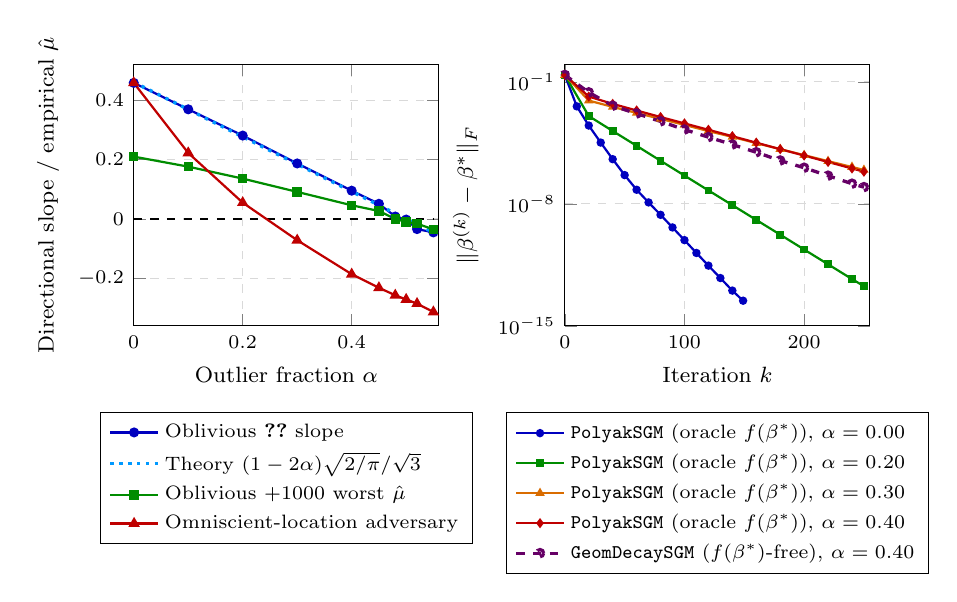
\begin{tikzpicture}
  \begin{groupplot}[
    group style={group size=2 by 1, horizontal sep=1.6cm},
    width=0.45\textwidth,
    height=4.9cm,
    grid=major,
    grid style={dashed,gray!30},
    tick label style={font=\scriptsize},
    label style={font=\footnotesize}
  ]
  \nextgroupplot[
    xlabel={Outlier fraction $\alpha$},
    ylabel={Directional slope / empirical $\hat\mu$},
    xmin=0, xmax=0.56,
    ymin=-0.36, ymax=0.52,
    legend style={at={(0.5,-0.33)}, anchor=north, legend columns=1, font=\scriptsize, cells={anchor=west}}
  ]
    \addplot[black, dashed, thick, domain=0:0.55, forget plot] {0};
    \addplot[blue!75!black, thick, mark=*, mark size=1.4pt] coordinates {
      (0.00, 0.4582) (0.10, 0.3691) (0.20, 0.2807) (0.30, 0.1868)
      (0.40, 0.0950) (0.45, 0.0509) (0.48, 0.0080) (0.50, -0.0022)
      (0.52, -0.0343) (0.55, -0.0454)
    };
    \addlegendentry{Oblivious \cref{prop:converse} slope}
    \addplot[blue!40!cyan, dotted, very thick, domain=0:0.55] {(1 - 2*x)*0.4607};
    \addlegendentry{Theory $(1-2\alpha)\sqrt{2/\pi}/\sqrt{3}$}
    \addplot[green!55!black, thick, mark=square*, mark size=1.3pt] coordinates {
      (0.00, 0.2098) (0.10, 0.1760) (0.20, 0.1357) (0.30, 0.0910)
      (0.40, 0.0459) (0.45, 0.0267) (0.48, -0.0002) (0.50, -0.0102)
      (0.52, -0.0161) (0.55, -0.0352)
    };
    \addlegendentry{Oblivious $+1000$ worst $\hat\mu$}
    \addplot[red!75!black, thick, mark=triangle*, mark size=1.6pt] coordinates {
      (0.00, 0.4582) (0.10, 0.2222) (0.20, 0.0547) (0.30, -0.0717)
      (0.40, -0.1862) (0.45, -0.2319) (0.48, -0.2572) (0.50, -0.2714)
      (0.52, -0.2853) (0.55, -0.3135)
    };
    \addlegendentry{Omniscient-location adversary}

  \nextgroupplot[
    ymode=log,
    xlabel={Iteration $k$},
    ylabel={$\Fnorm{\beta^{(k)} - \beta^*}$},
    xmin=0, xmax=255,
    ymin=1e-15, ymax=1,
    legend style={at={(0.5,-0.33)}, anchor=north, legend columns=1, font=\scriptsize, cells={anchor=west}}
  ]
    \addplot[blue!75!black, thick, mark=*, mark size=1.1pt] coordinates {
      (0, 2.50e-1) (10, 3.96e-3) (20, 3.14e-4) (30, 3.30e-5) (40, 3.68e-6)
      (50, 4.48e-7) (60, 6.46e-8) (70, 1.21e-8) (80, 2.35e-9) (90, 4.42e-10)
      (100, 8.28e-11) (110, 1.52e-11) (120, 2.85e-12) (130, 5.53e-13)
      (140, 1.05e-13) (149, 2.76e-14)
    };
    \addlegendentry{\texttt{PolyakSGM} (oracle $f(\beta^*)$), $\alpha = 0.00$}
    \addplot[green!55!black, thick, mark=square*, mark size=1.0pt] coordinates {
      (0, 2.50e-1) (20, 1.10e-3) (40, 1.53e-4) (60, 2.15e-5) (80, 2.99e-6)
      (100, 4.21e-7) (120, 5.94e-8) (140, 8.47e-9) (160, 1.20e-9)
      (180, 1.71e-10) (200, 2.40e-11) (220, 3.40e-12) (240, 4.82e-13) (250, 1.88e-13)
    };
    \addlegendentry{\texttt{PolyakSGM} (oracle $f(\beta^*)$), $\alpha = 0.20$}
    \addplot[orange!85!black, thick, mark=triangle*, mark size=1.2pt] coordinates {
      (0, 2.50e-1) (20, 8.49e-3) (40, 3.69e-3) (60, 1.66e-3) (80, 7.52e-4)
      (100, 3.41e-4) (120, 1.51e-4) (140, 6.95e-5) (160, 3.07e-5)
      (180, 1.39e-5) (200, 6.27e-6) (220, 2.84e-6) (240, 1.31e-6) (250, 8.83e-7)
    };
    \addlegendentry{\texttt{PolyakSGM} (oracle $f(\beta^*)$), $\alpha = 0.30$}
    \addplot[red!75!black, thick, mark=diamond*, mark size=1.2pt] coordinates {
      (0, 2.50e-1) (20, 1.45e-2) (40, 5.48e-3) (60, 2.30e-3) (80, 9.67e-4)
      (100, 4.17e-4) (120, 1.79e-4) (140, 7.68e-5) (160, 3.26e-5)
      (180, 1.38e-5) (200, 5.92e-6) (220, 2.54e-6) (240, 1.08e-6) (250, 7.02e-7)
    };
    \addlegendentry{\texttt{PolyakSGM} (oracle $f(\beta^*)$), $\alpha = 0.40$}
    \addplot[violet!80!black, dashed, very thick, mark=o, mark size=1.3pt] coordinates {
      (0, 2.50e-1) (20, 2.51e-2) (40, 4.26e-3) (60, 1.53e-3) (80, 5.42e-4)
      (100, 1.84e-4) (120, 6.77e-5) (140, 2.54e-5) (160, 9.13e-6)
      (180, 3.07e-6) (200, 1.18e-6) (220, 4.12e-7) (240, 1.43e-7) (250, 9.11e-8)
    };
    \addlegendentry{\texttt{GeomDecaySGM} ($f(\beta^*)$-free), $\alpha = 0.40$}
  \end{groupplot}
\end{tikzpicture}

  \caption{Left (Experiment~B, $d=10, r=3, m=500$): Oblivious-support outliers preserve positive local sharpness up to $\alpha < 1/2$ and cross zero near $\alpha = 0.50$, whereas an omniscient-location adversary breaks local optimality strictly below $\alpha = 0.30$. Right (Experiment~D, $d=20, r=3, m=500$): Local trajectories from $\Fnorm{\beta^{(0)} - \beta^*} = 0.25$ under $\pm 100$ oblivious corruptions for oracle-$f(\beta^*)$ \texttt{PolyakSGM} ($\alpha \in \{0, 0.2, 0.3, 0.4\}$) alongside $f(\beta^*)$-free \texttt{GeomDecaySGM} ($\lambda_k = 0.04 \cdot 0.95^k$) at $\alpha = 0.40$; see Supplement~SM2 (Table~SM3) for 5-seed statistics.}
  \label{fig:outliers-polyak}
\end{figure}

\begin{figure}[t]
  \centering
  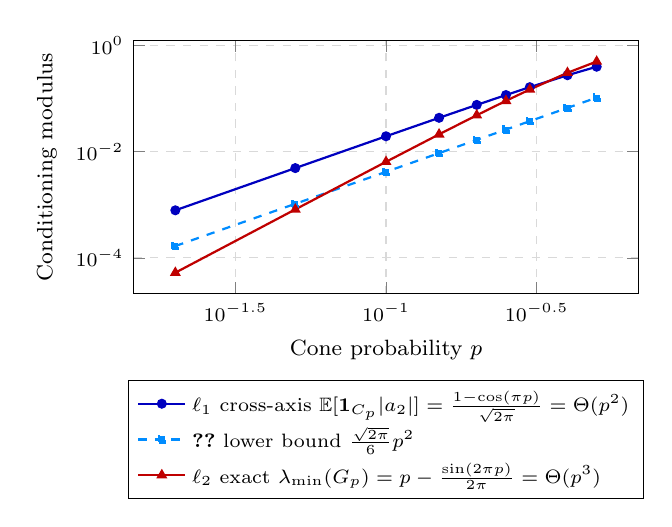
\begin{tikzpicture}
  \begin{loglogaxis}[
    width=0.66\textwidth,
    height=4.8cm,
    xlabel={Cone probability $p$},
    ylabel={Conditioning modulus},
    grid=major,
    grid style={dashed,gray!30},
    tick label style={font=\scriptsize},
    label style={font=\footnotesize},
    legend style={at={(0.5,-0.34)}, anchor=north, legend columns=1, font=\scriptsize, cells={anchor=west}}
  ]
    \addplot[blue!75!black, thick, mark=*, mark size=1.4pt] coordinates {
      (0.02, 7.872e-4) (0.05, 4.912e-3) (0.10, 1.953e-2) (0.15, 4.348e-2)
      (0.20, 7.619e-2) (0.25, 1.168e-1) (0.30, 1.644e-1) (0.40, 2.757e-1) (0.50, 3.989e-1)
    };
    \addlegendentry{$\ell_1$ cross-axis $\E[\ind_{C_p}|a_2|] = \frac{1-\cos(\pi p)}{\sqrt{2\pi}} = \Theta(p^2)$}
    \addplot[blue!45!cyan, dashed, thick, mark=square*, mark size=1.1pt] coordinates {
      (0.02, 1.671e-4) (0.05, 1.044e-3) (0.10, 4.178e-3) (0.15, 9.400e-3)
      (0.20, 1.671e-2) (0.25, 2.611e-2) (0.30, 3.760e-2) (0.40, 6.684e-2) (0.50, 1.044e-1)
    };
    \addlegendentry{\cref{lem:bathtub} lower bound $\frac{\sqrt{2\pi}}{6}p^2$}
    \addplot[red!75!black, thick, mark=triangle*, mark size=1.5pt] coordinates {
      (0.02, 5.260e-5) (0.05, 8.184e-4) (0.10, 6.451e-3) (0.15, 2.124e-2)
      (0.20, 4.863e-2) (0.25, 9.085e-2) (0.30, 1.486e-1) (0.40, 3.065e-1) (0.50, 5.000e-1)
    };
    \addlegendentry{$\ell_2$ exact $\lambda_{\min}(G_p) = p - \frac{\sin(2\pi p)}{2\pi} = \Theta(p^3)$}
  \end{loglogaxis}
\end{tikzpicture}

  \caption{Analytical $\ell_1$ versus $\ell_2$ active-cone conditioning on narrow 2D cones $C_p$ (\cref{prop:l1-vs-l2}): $\alpha_{\ell_1}(C_p) = \Theta(p^2)$ improves by a full factor of $p$ over $\lambda_{\min}(G_p) = \Theta(p^3)$.}
  \label{fig:cones}
\end{figure}

% ============================================================================
\section{Discussion and Limitations}
\label{sec:discussion}
% ============================================================================

Five open limitations merit further investigation:
\begin{enumerate}
  \item \textbf{Local versus global finite-sample sharpness.} \Cref{thm:pop-r2} is global for $r = 2$, whereas \cref{thm:main-finite} is local on $B(\beta^*, \rho)$ and does not exclude higher-valued spurious local minima. Proving global finite-sample sharpness for $r = 2$ and establishing provable robust initialization for $r \ge 3$ remain open.
  \item \textbf{Sample complexity in $r$ and $\pi_{\min}$.} \Cref{thm:main-finite} requires $m \gtrsim \frac{d}{\gamma^2}\log\frac{1}{\gamma} + \frac{rd}{\gamma}\log\frac{r}{\gamma}$, which via $\alpha_{\min} \ge \frac{\sqrt{2\pi}}{6}\pi_{\min}^2$ yields $\tilde O(d/\pi_{\min}^4)$ samples, whereas \cite[Section~5.2.2; Figure~5 in arXiv:2201.04611]{charisopoulos2024superpolyak} and \cref{tab:dim-kappa} suggest $m = O(rd)$ suffices empirically. Tightening the cone-concentration term (e.g., via Mendelson's small-ball method) remains open.
  \item \textbf{Oblivious versus omniscient outlier support.} \Cref{thm:main-finite} requires $S_{\mathrm{bad}}$ to be independent of $A$ (allowing arbitrary $\xi_i(A)$). Quantifying the exact omniscient-support breakdown threshold $\alpha_{\mathrm{omni}}(\pi_{\min})$ is left for future work.
  \item \textbf{Gaussian design and quantitative $(b)$-regularity.} Our polar wedge integrals and Lean~4 formalization rely on $a_i \sim \mathcal{N}(0, I_d)$. Extending \cref{thm:main-finite} to isotropic sub-Gaussian designs and deriving quantitative $(b)$-regularity constants $(C_{(b)}, \eta_{(b)})$ for \cref{cor:superpolyak} are natural next steps.
  \item \textbf{Unpublished overlap with alternating LAD methods.} As noted in \cref{sec:intro}, Kim, Kanj, and Lee \cite{kim2024mds,kim2024thesis} announced an alternating LAD / Gauss--Newton approach for robust max-affine regression (extending \cite{kim2025robustpr}), with proofs not yet publicly available. Because finite-sample proofs for alternating LAD methods may share underlying active-cone and wedge-flip concentration tools, the exact degree of overlap cannot be determined until a full published analysis appears.
\end{enumerate}

% ============================================================================
\appendix
\section{Supplemental Elementary Lemmas}
\label{app:proofs}
% ============================================================================

\begin{lemma}[Exact 1D trigonometric wedge integral]
  \label{lem:trig-wedge}
  For all $c_1, c_2 > 0$ and $\theta \in (0, \pi)$,
  \[
    \int_0^\theta \min\bigl(c_1 \sin\psi,\, c_2 \sin(\theta - \psi)\bigr)\,d\psi
    = c_1 + c_2 - \sqrt{c_1^2 + c_2^2 + 2c_1 c_2 \cos\theta}.
  \]
\end{lemma}
\begin{proof}
Set $R := \sqrt{c_1^2 + c_2^2 + 2c_1 c_2 \cos\theta} > 0$, and define $\psi^* \in (0, \theta)$ by $\cos\psi^* = \frac{c_1 + c_2\cos\theta}{R}$ and $\sin\psi^* = \frac{c_2\sin\theta}{R} > 0$, so $\cos(\theta - \psi^*) = \frac{c_2 + c_1\cos\theta}{R}$. Since $c_1\sin\psi - c_2\sin(\theta - \psi) = R\sin(\psi - \psi^*)$ switches sign at $\psi^*$, direct integration gives $c_1(1 - \cos\psi^*) + c_2(1 - \cos(\theta - \psi^*)) = c_1 + c_2 - R$.
\end{proof}

\begin{lemma}[Numerical bound for the $(1/6)$-net operator-norm tail]
  \label{lem:op-num}
  For all integers $m, d \ge 0$ with $32d \le m$, $13^d \bigl(\frac{5}{3}e^{-8/9}\bigr)^m \le e^{-9m/32}$.
\end{lemma}
\begin{proof}
Mirroring the Lean~4 lemma \texttt{thirteen\_pow\_d\_mul\_chisq\_le}: (i)~$e \ge \sum_{j=0}^5 \frac{1}{j!} = \frac{163}{60}$ gives $13(\frac{5}{3})^{32} \approx 1.633 \times 10^8 \le (\frac{163}{60})^{19} \approx 1.778 \times 10^8 \le e^{19} \le e^{175/9}$, so $13(\frac{5}{3}e^{-8/9})^{32} \le e^{-9}$; (ii)~$e^{175/288} \ge 1 + \frac{175}{288} + \frac{1}{2}(\frac{175}{288})^2 \ge 1.792 > \frac{5}{3}$ gives $\frac{5}{3}e^{-8/9} \le e^{-9/32}$. Writing $m = 32d + k$ ($k \ge 0$) yields $13^d(\frac{5}{3}e^{-8/9})^{32d+k} \le e^{-9d}e^{-(9/32)k} = e^{-9m/32}$.
\end{proof}

\begin{lemma}[Radial Gaussian moments and Bernstein induction]
  \label{lem:moment-ind}
  For every integer $p \ge 0$, $\int_0^\infty r^{p+1} e^{-r^2/2}\,dr = 2^{p/2}\Gamma(1 + p/2)$. Moreover, for every integer $p \ge 2$, $2^{3p/2}\Gamma(1 + p/2) \le p!\,2^p$.
\end{lemma}
\begin{proof}
The integral identity holds at $p = 0, 1$ and follows by integration by parts. For the inequality, induct by steps of~$2$: at $p = 2$, $2^3\Gamma(2) = 8 = 2!\,2^2$; at $p = 3$, $2^{9/2}\Gamma(5/2) = 12\sqrt{2\pi} < 31 < 48 = 3!\,2^3$; passing from $p \ge 2$ to $p + 2$ multiplies the left-hand side by $4(p + 2)$ and the right-hand side by $4(p + 1)(p + 2) \ge 12(p + 2)$.
\end{proof}

\section*{Acknowledgments and Declarations}
\textbf{Disclosure of Artificial Intelligence Use.} The author discloses that generative AI tools (autonomous LLM-based research assistants, together with human-initiated adversarial review via separate LLM sessions) participated substantively across this project, including research problem exploration, mathematical theorem formulation, proof development and revision, literature retrieval, Lean~4 formalization, Python coding and numerical experiments, and manuscript drafting and formatting. No AI tool is listed as an author. To independently verify core reasoning steps, \cref{thm:pop-r2,thm:main-finite}, \cref{lem:flip-decomp,lem:bathtub,lem:op-norm,lem:cone-conc,lem:flip-conc}, \cref{lem:trig-wedge,lem:op-num,lem:moment-ind}, and \cref{prop:converse} were machine-checked by the Lean~4 kernel (\texttt{v4.35.0}, zero \texttt{sorry}s, standard axioms only; Supplement~SM1). Pen-and-paper results outside the Lean kernel are explicitly itemized in Supplement~SM1. This document is an unrefereed research preprint.

\medskip
\noindent\textbf{Code, Archival Materials, and Conflict of Interest.} The companion Lean~4 formal verification package, reproducible experiment scripts, and audit records are available at \url{https://github.com/Vesaluna/sharp-growth-max-linear-regression}. The author declares no competing financial or non-financial interests.

\bibliographystyle{abbrvnat}
\bibliography{references}

\end{document}
